%%%%%%%%%%%%%%%%%%%%%%% file typeinst.tex %%%%%%%%%%%%%%%%%%%%%%%%%
%
% This is the LaTeX source for the instructions to authors using
% the LaTeX document class 'llncs.cls' for contributions to
% the Lecture Notes in Computer Sciences series.
% http://www.springer.com/lncs       Springer Heidelberg 2006/05/04
%
% It may be used as a template for your own input - copy it
% to a new file with a new name and use it as the basis
% for your article.
%
% NB: the document class 'llncs' has its own and detailed documentation, see
% ftp://ftp.springer.de/data/pubftp/pub/tex/latex/llncs/latex2e/llncsdoc.pdf
%
%%%%%%%%%%%%%%%%%%%%%%%%%%%%%%%%%%%%%%%%%%%%%%%%%%%%%%%%%%%%%%%%%%%


\documentclass[conference]{IEEEtran}

% *** GRAPHICS RELATED PACKAGES ***
%
\ifCLASSINFOpdf
  % \usepackage[pdftex]{graphicx}
  % declare the path(s) where your graphic files are
  % \graphicspath{{../pdf/}{../jpeg/}}
  % and their extensions so you won't have to specify these with
  % every instance of \includegraphics
  % \DeclareGraphicsExtensions{.pdf,.jpeg,.png}
\else
  % or other class option (dvipsone, dvipdf, if not using dvips). graphicx
  % will default to the driver specified in the system graphics.cfg if no
  % driver is specified.
  % \usepackage[dvips]{graphicx}
  % declare the path(s) where your graphic files are
  % \graphicspath{{../eps/}}
  % and their extensions so you won't have to specify these with
  % every instance of \includegraphics
  % \DeclareGraphicsExtensions{.eps}
\fi

\usepackage{bbding}

\usepackage{wrapfig}
\usepackage{threeparttable}
\usepackage{amssymb,amsmath}
\setcounter{tocdepth}{3}
%\usepackage{verbatim}
\usepackage{graphicx}
\usepackage{subfigure}
%\usepackage[ruled,vlined]{algorithm2e}
\usepackage[noend]{algpseudocode}
\usepackage{algorithmicx,algorithm}
\usepackage{url}
\usepackage{color}
%\usepackage{verbatim}
\usepackage{multicol}
\usepackage{lipsum}
\usepackage{xspace}
\newsavebox{\tablebox}
\usepackage{multirow}
\usepackage{setspace}
%\usepackage{enumitem}
\usepackage{paralist}
\let\itemize\compactitem
\let\enditemize\endcompactitem
\let\enumerate\compactenum
\let\endenumerate\endcompactenum
\let\description\compactdesc
\let\enddescription\endcompactdesc
%\pltopsep=0pt%\medskipamount
%\plitemsep=0pt
%\plparsep=0pt
%
%%=============added by Rj to reduce space
\setlength{\parskip}{1pt}
\newcommand{\marginremark}[2]{\annotatedmarginremark{\clubsuit}{$\clubsuit$}{#1}{#2}}
\newcommand{\rjnote}{\color{red}}
\newcommand{\ccnote}[1]{\marginremark{CH}{#1}}
%\newcommand{\rjnote}[1]{\marginremark{RJ}{#1}}
\def\mathbi#1{\textbf{\em #1}}
 \newcommand{\comment}[1]{}
  \newcommand{\sig}[1]{\textsf{{\small #1}}}
  \newcommand{\nn}{\mathbb{N}}
\newcommand{\bool}{\mathbb{B}}
%\theoremstyle{definition}
\newtheorem{proposition}{Proposition}
\newtheorem{defi}{Definition}

\hyphenation{op-tical net-works semi-conduc-tor}
\begin{document}

%\mainmatter  % start of an individual contribution

% first the title is needed
\title{A hybrid algorithm for multi-objective mapping and scheduling optimization of MPSoCs}
% a short form should be given in case it is too long for the running head

% the name(s) of the author(s) follow(s) next
%
% NB: Chinese authors should write their first names(s) in front of
% their surnames. This ensures that the names appear correctly in
% the running heads and the author index.
%


%\author{
%
%\IEEEauthorblockN{Rongjie Yan\IEEEauthorrefmark{1},  Yupeng Zhou\IEEEauthorrefmark{2},   Yige Yan\IEEEauthorrefmark{2}, Minhao Yin\Envelope\IEEEauthorrefmark{2}, Min Yu\IEEEauthorrefmark{3}, Chih-Hong Cheng\IEEEauthorrefmark{4},  Feifei Ma\IEEEauthorrefmark{1}, Kai Huang\IEEEauthorrefmark{3}}
%\IEEEauthorblockA{\IEEEauthorrefmark{1}State Key Laboratory of Computer Science, Institute of Software, Beijing, China
%}
%\IEEEauthorblockA{\IEEEauthorrefmark{2}Schlool of Computer Science and Information Technology, Northeast Normal University, Changchun, China
%}
%\IEEEauthorblockA{\IEEEauthorrefmark{3}Department of ISEE, Zhejiang University, Hangzhou, China
%}
%\IEEEauthorblockA{\IEEEauthorrefmark{4}Fortiss - An-Institut der TU M\"{u}nchen, Munich, Germany 
%}
%\IEEEauthorblockA{\{yrj, maff\}@ios.ac.cn; \{zhouyp605,yanyg270,ymh\}@nenu.edu.cn;\{11131030,huangk\}@zju.edu.cn;cheng@fortiss.org
%}
%}
\maketitle
\begin{abstract}
Multi-processors are widely used in embedded systems. The resource limitation requires designers to find optimizations among various design considerations. In this paper, we model tradeoffs between makespan and the balance of processor workloads for the problem of tasks mapping and scheduling in a multi-processor environment. To encode the effect of precedence relations between different tasks in scheduling, the model also considers communication cost in the formulation. Furthermore, to approximate the Pareto front of the multi-objective optimization problem, we propose a multi-objective hybrid algorithm(MOHA) by integrating pareto local search into an evolutionary process. We evaluate the efficiency of the method on a series of benchmarks and compare the results with existing multi-objective optimization methods. Experimental results show that the proposed algorithm can obtain better solutions for various real-world cases, compared with state-of-the-art methods.

 \end{abstract}
%\tableofcontents
\vspace{-5pt}
\section{Introdution\label{se:intro}}
Mapping and scheduling applications onto a multi-core platform is a key factor, to cope with continuously
increasing conflicting demands of both high performance and low power consumption. %The requirements are always conflicting with each other. 
For example, makespan minimization requires allocating more computations on faster processors. Consequently, the unbalanced workload may keep fast processors busy in computation, while other processors being waiting, which leads to more power consumption. On the other hand, computation workload balance leads to a more parallel implementation. However, the increasing communication between tasks on different processors may result in the increase in the makespan. Therefore, there exists a set of mutually incomparable solutions representing different design tradeoffs.

To achieve high performance and low power consumption for MPSoCs, we consider workload balance and makespan minimization in static task allocation and scheduling problems. Meanwhile, we model the corresponding constraints together, to avoid local optimal obtained from separated optimization of the two criteria.

In this context, the traditional solution for mapping and scheduling problems with integer linear programming (ILP), is less feasible to cope with multiple objectives and large scale systems~\cite{DBLP:journals/jcp/YaoZW14,HuangYYZYBJF15}. There are various algorithms and heuristics for computing solutions for multi-objective optimization problems. For example, evolutionary algorithms~\cite{Yang2009,konak2006multi},  based on successive optimization and simulation steps, use heuristics to refine optimal solutions.
Some constraint solvers are also applied to approximate the Pareto fronts and guarantee the computable bounds~\cite{legriel2010approximating}.
%To speed up the optimization progress, a problem can be decomposed and consecutively solved~\cite{kang2012multi}.
However, the efficiency and scalability are still the bottlenecks for the methods to be applied for large scale applications.
%\cite{legriel2010approximating} submits queries to a constraint solver, and use the answers as the approximation of  the Pareto front of the problem, or the guarantee of the computable bounds.
To tackle this problem, we propose an alternative method, % to solve the problem, 
which is based on a mixture of multi-objective genetic and local search techniques. By integrating a pareto local search  into an evolutionary procedure, we could obtain both the expansive searching ability of the population-based technique and the intensive searching ability of the local search method.
Specifically, the proposed algorithm mainly consists of three ingredients, including a problem-specific initialization to generate promising initial candidate solutions, a genetic operator to roughly search the space, and a local search operator to exhaustively seek through the better feasible solutions.% In order to test the effectiveness of the algorithm, we have tested it against realistic benchmarks and also compared with other optimization algorithms, such as NSGAII.

Compared with the-state-of-the-art methods, the algorithm is more efficient for computing Pareto optimals, and is capable of dealing with large scale realistic applications.
%We evaluate the efficiency of the algorithm for mapping and scheduling optimization of MPSoCs according to the makespan and workload balance minimization. Compared with the-state-of-the-art methods, for the similar solutions, the algorithm requires less time {\rjnote and memory(is that ok? Shall we remove this?)}, which is capable of optimization of large-scale realistic applications.


The contributions are as follows. First, we propose to optimize task allocation and scheduling of MPSoCs with respect to two criteria, i.e., makespan minimization and workload balance, involving both performance and energy consumption considerations. Second, to avoid local optimization from stepwise methods or decomposition methods, we model the constraints on mapping and scheduling together. The model characterizes computation, inter-processor communication, and can be extended for other optimization criteria. Finally, to provide solutions for realistic applications,        we propose a Pareto local search based algorithm within a novel genetic framework, called Multi-objective hybrid algorithm(MOHA), to approximate Pareto optimal. Experimental results show that
we could obtain the solutions even for realistic applications with more than two hundred tasks.
%This local search technique blending with a novel genetic framework is a balance between exploration and exploitation. Moreover, experimental results show that the PMA provides not only abundant but also high-quality candidates for decision makers}. Second, we have modeled the constraints of the mapping and scheduling problem. Benefited from the algorithm, we could obtain the solutions from two-objective optimizaiton even for realistic applications with more than two hundred tasks.

The paper is structured as follows. After a brief summary of the related work, we define task graphs for application models, provide the assumption for target platforms, and describe the mapping and scheduling problem in Seciton \ref{se:pre}. Section \ref{se:ilp} models constraints for mapping and scheduling problem.
Section \ref{se:loc} introduces MOHA algorithm.
We present the experimental results in Section \ref{se:imp}. Section \ref{se:con} concludes.

%\vspace{-5pt}
\vspace{-2pt}
\section{Related work\label{se:re}}
Optimizations on computation, communication, throughput and energy consumption are always conflicting~\cite{lin2012communication,IEICE14,FM15}. When facing multiple objectives, a solution is to formulate objectives with different weights~\cite{IEICE14}, thus transforming multi-objective into one to be solved with integer linear solvers.
However, the shortage of scalability limits its application for realistic problems.
The alternative methods, such as stepwised optimization~\cite{IEICE14}, the integration of evolutionary algorithms~\cite{lin2012communication}, may still fall into the problem of local optimization, and the results may not be real Pareto fronts.

Search based algorithms are also considered in the literature for mapping and scheduling optimization of MPSoCs. Zhu et. al. model the constraints and task dependency into timed automata and compute Pareto front with model checking techniques~\cite{FM15}.
\cite{legriel2010approximating} provides a multi-dimensional binary search algorithm for approximating the Pareto fronts and guaranteeing the computable bounds. These techniques also suffer from scalability problems.

To obtain Pareto optimal for large scale systems, \cite{thiele2007mapping} addresses the mapping problems with multiple optimization objectives, based on evolutionary algorithms. \cite{yassa2013genetic} applies genetic algorithms for multi-objective optimization in workflow scheduling. Among the techniques, the Non-dominated Sorting Genetic Algorithm (NSGAII)~\cite{deb2002fast} is recognized as one of the most classical framework for multi-objective optimization problems. %Addition to these methods,
%\cite{tetzlaffintelligent} applies machine learning technique to learn the program behaviour and provides communication and power-efficient mapping strategies.
In this setting, initial solution and heuristics are important factors for the efficiency of the algorithms. On the other hand, local search based methods have achieved great success in solving various combinatorial problems by obtaining near-optimal solutions with a small cost~\cite{wang2016two}. Therefore, the aim of this paper is to integrate a local search technique into a genetic framework to improve both the efficiency and accuracy when computing Pareto optimals.

%\textbf{Real-world issues are often incomputable by exact methods which waste much time. Then local search approaches are introduced accordingly and proved to be significant for combinatorial optimization problems. Local search techniques~\cite{Ishibuchi98} are always applied to solve flowshop scheduling problems.  \cite{lourencco2003iterated} firstly proposes an iterated local search in which a perturbation is applied to the solution generated by the last search phase. Subsequently, \cite{hansen2003variable} developed a time-saving local search called variable neighbourhood search, aming to reduce the searching space. In recent years, many researchers focus on extensions of the local search for multi-objective problems. \cite{moalic2013fast} proposed a fast local search approach for multi-objective problems based on pareto optimal. Although optimal solutions cannot be guaranteed by local search methods, near-optimal solutions can be obtained with reasonable time. This characteristic is of importance especially for large-scale problems.}


\section{Preminaries\label{se:pre}}

This section first defines the concept of an application model to be mapped and scheduled. Further, the assumption of the target platform is presented. Finally, the problem to be optimized
is sketched.
\subsection{Weighted task graph}
In this paper, we concern coarse-grained application models. An application consists of a set of tasks with well-defined precedence constraints. Therefore, we adopt task graphs as the formulation~\cite{cotton2011multi}. To record the amount of work to be dealt with on a task, and data to be transferred, we assign weights on the tasks and data flows between different tasks, respectively.
\begin{defi}[Weighted Task Graph]
A weighted task graph is a tuple $G=\langle T,E\rangle$, where $T$ is a finite set of tasks, with $\delta: T\rightarrow \nn$ to indicate the amount of work to be dealt with on each task, and $E\subseteq T\times T$ is a set of precedence relations with $c: E\rightarrow \nn$ to indicate the amount of data transferred between each pair of tasks.
\end{defi} 

\begin{figure}
\centering
 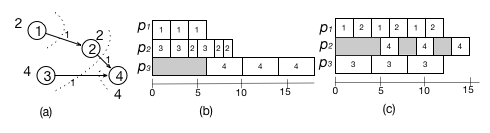
\includegraphics[width=0.85\columnwidth]{figures/taskgraph}
  \caption{A running example.}
 \label{fig:taskgraph}
 \vspace{-6.5mm}
 \end{figure}
 If there is no explicit precedence relation between a pair of tasks, the amount of communicated data is zero.  
 We also assume that the graph is acyclic. For an application with loops, we need to reduce it to acyclic graph by unfolding techniques. Take the model in Fig.~\ref{fig:taskgraph} as an example. There are four tasks, each of which is labelled with the amount of work, and three edges are labeled with the amount of transfered data. 

\subsection{Target platform}
We consider architectures connected with heterogeneous processors, each of which has a private memory, as shown in Fig.\ref{fig:platform}. Each processor can access its private memory directly, while accessing private memories of peer processors is not permitted. In order to communicate with peer processors, DMAs (Direct Memory Access) are implemented in the hardware platform. They can read from and write to all private memories under the control of processors. % each processor can access others through buses. %The DMA module takes charge of communication between the processors and off-memory. 
\begin{figure}
\centering
 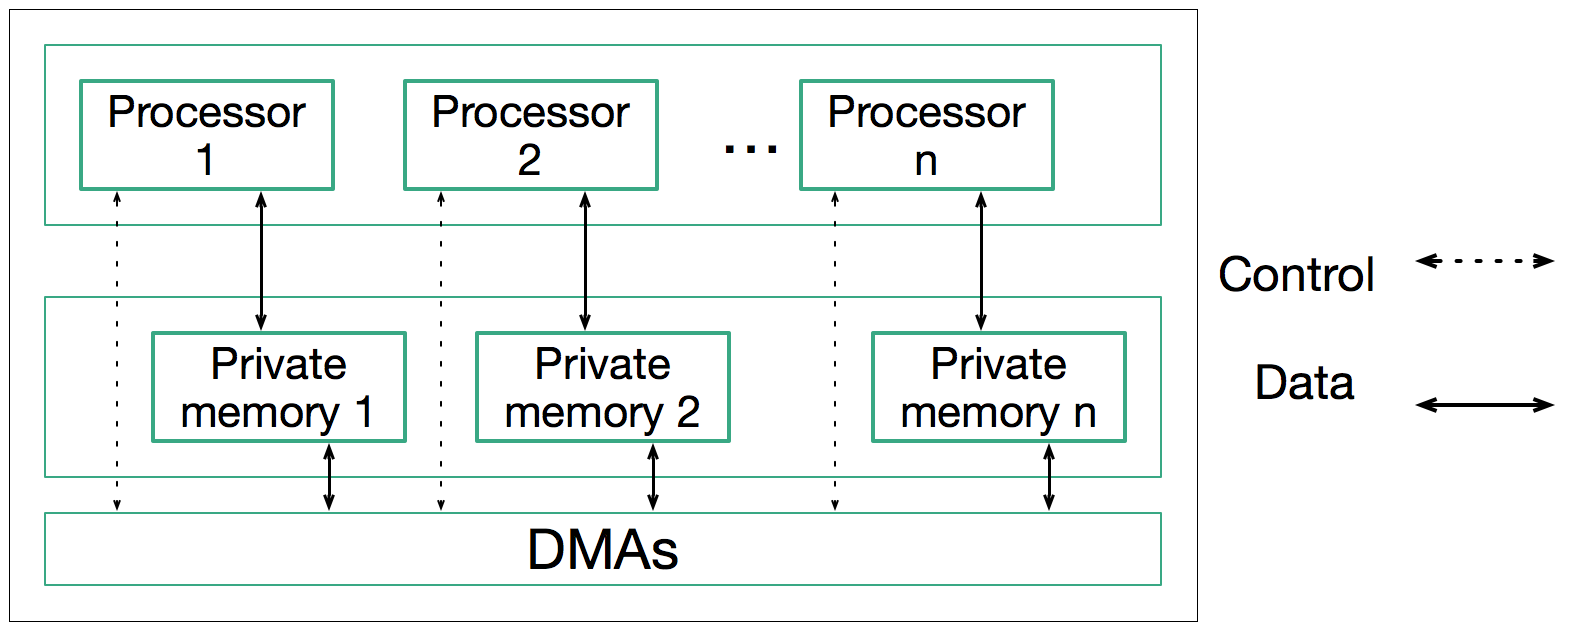
\includegraphics[width=0.8\columnwidth]{figures/platform.png}
  \caption{The target architecture.}
 \label{fig:platform}
 \vspace{-7.5mm}
 \end{figure}
We make the following assumptions for the target architecture:
\begin{enumerate}
%\item The architecture is fully connected.%, such that all the processors and the shared bus can be reached via any buses.
\item The cost for intra-processor communication is negligible. We only consider inter-processor communication.
\item A processor is occupied for initializing communication. Once the initialization is ready, the processor is released.
\item An inter-processor communication can start after the initialization. And multiple transmission to different destinations can be executed simultaneously. 
\item There is no memory access collisions.
\item Private memories are big enough for data storage.
\end{enumerate}

When the weight of a precedence relation in a task graph is greater than zero, and the two tasks are allocated to different processors, inter-processor communication is required. To simplify the model description, we restrict the communication architecture to a direct connection between different processors via inter-processor communication.

%To simplify the description of the constraints, we ignore the cost of task switch within the same processor.
\vspace{-8pt}
\subsection{Problem description}

%Given a task graph and a set of processors, 
We aim to construct static schedules for the target implementation. 
More precisely, the
tasks are statically allocated among the processors and
all executions (instances) of a task are executed on the same
processor, and no instance is permitted to migrate among
processors. Hence, mapping relations between tasks and processors are fixed during execution, and the sequences of task execution remain unchanged.

The tasks of an application will be repeatedly executed for a certain scenario.
%And the scheduling may be optimized after several iterations. 
Therefore, it is not enough to estimate the makespan of the whole with one time execution of the tasks. 
And we consider the minimisation of makespan within certain number of iterations. 


Given a task graph $G$ and a set of processors $P$, a mapping is a function $m: T \times P\rightarrow \bool$ with $m(t_i,p_k)=true$ meaning that task $t_i$ executes on processor $p_k$. 
Then the scheduling of tasks is a function $\tau: T\times \nn \rightarrow \nn$ with $\tau(t_i,u)=n$ meaning that the time of $u$th invocation of task $t_i$ is $n$. Suppose the function of processor speeds is $\rho: P\rightarrow \nn$. The duration of executing $t_i$ is $\kappa(t_i)=\delta(t_i)/(\sum^{|P|}_{k=1}\rho(k)*m(t_i,p_k))$. By abuse of notation, $\tau(t_i,u)$ is denoted by $\tau^u_i$ and others only use the subscripts instead. Then given the number of iterations $N$, the makespan is 
$${\cal{M}}=max \{i : \forall i ~\tau^N_i + \kappa_i\}.$$ 
The ideal situation for a balanced workload is that the workload on each processor is equal, i.e., 
%$\alpha=\dfrac{1}{|P|}*\sum^{|P|}_{k}  (\sum^{|T|}_{i} \delta_i *m_{i,k})/ \rho_k$. 
$aver= \sum^{|T|}_{i=1} \delta_i /|P|$. 
Hence, the difference between real workloads and the perfectly balanced workload is measure with $${\cal{W}}=\sum^{|P|}_{k=1} \mid\sum^{|T|}_{i=1}\delta_i*m_{i,k}- aver\mid.$$

Consider the example in Fig.~\ref{fig:taskgraph} again. There are three processors, where the speed of $p_2$ is twice as fast as that of $p_1$ and $p_3$.  
In Fig.~\ref{fig:taskgraph}(b),
tasks 1 and 4 are mapped to processors $p_1$ and $p_3$, respectively, and tasks 2 and 3 are allocated to $p_2$.
If we ignore the cost for communication initialization, the makespans of first and third iterations in Fig.~\ref{fig:taskgraph}(b) are 10 and 18 respectively. If we change the allocation to Fig.~\ref{fig:taskgraph}(c), we can obtain a more balanced workload with a smaller makespan.

%\cite{DBLP:journals/jcp/YaoZW14} considers the existence of DMA for transmission optimization. Both data and task parallelism are encoded in the constriants for mapping and scheduling optimization.\cite{yang2008ilp}. 

\section{Constraint formulations\label{se:ilp}}
In this section, for the problem of mapping and scheduling of an application on certain platforms, we formalize it as an integer linear programming model, which is the input of our algorithm.
The model mainly constructs constraints on scheduling, with respect to computation effort.
 To measure the introduced communication cost for workload balance and its effect to the makespan, we also consider the inter-processor communication in the optimization of the two objectives. To simplify the modelling, we assume that a task can start execution once the corresponding communication is finished. 

\subsection{Parameters and variables}
Given a model $G=\langle T, E\rangle$ and a set of processors $P$, the input parameters to the ILP model is summarized in Table \ref{tab:par}.
\begin{table}[t]\centering
\caption{Input of the ILP model\label{tab:par}}
\begin{tabular}{ll}\hline
Notation & Definition \\\hline
	 $N$ & The number of executions for every task \\
	%$M$ & A big enough integer\\
	$a_{i,k}$ & Whether task $t_i$ can be mapped to processor $p_k$\\
	$d_{i,j}$ & Precedence relation between tasks $t_i$ and $t_j$\\
	 $c_{i,j}$ & The size of data transfer from task $t_i$ to $t_j$\\
	$\delta{i}$& The amount of work for task $t_i$\\
	$\eta$ & The cost for communication initialization\\
	\hline
\end{tabular}	
\end{table}

With the input parameters, the mapping and scheduling steps consist of 1) allocating each task to a unique processor; 2) scheduling the tasks mapped to different processors.
 Then the following decision variables can completely capture the allocation and scheduling information.
 \begin{itemize}
	\item $m_{i,k}$:  shows whether task $t_i$ is mapped to processor $p_k$;
	\item $q_{k,i,j}$: the execution sequence between tasks $t_i$ and $t_j$ on $p_k$;	
	\item $\tau^u_{i}$: the start time of task $t_i$ at $u$th iteration
	%\item $\Delta$: the makespan for all tasks finishing all iterations;	
\end{itemize}
To facilitate the modelling of constraints, we introduce the following auxiliary variables:
%\begin{itemize}
	1) $b_{i,j}$: indicates whether tasks $t_i$ and $t_j$ are mapped to the same processor;	2) $bp_{k,i,j}$: indicates whether tasks $t_i$ and $t_j$ are mapped to processor $p_k$;
	3) $o_{i,j}$: indicates whether inter-processor communication exists between tasks $t_i$ and $t_j$.
%\end{itemize}
These variables are used to check the existence of communication cost and the precedence executing sequence of tasks on same processors.

\subsection{Constraints}
To encapsulate both the mapping and scheduling solution restricted by the underlying target architecture, 
 we introduce two categories of constraints. %The first is on mapping, communication and the execution sequences of tasks. The second restricts the behaviors between executed tasks.
 
 The first category of constraints restricts the mapping of tasks on processors,  the inter-relation between dependent tasks, and tasks mapped on the same processors.
 	\begin{equation}\label{eq:1}
	\begin{array}{l} 
		\sum_{k=1}^{|P|}m_{i,k}==1, ~\textrm{ and }~m_{i,k} \leq a_{i,k} 
	\end{array}
	\end{equation}
	\begin{equation}\label{eq:2}
	\begin{array}{l} 
		%b_{i,i}==0 & \\
		b_{i,j}== 1-(\sum_{k=1}^{|P|} \mid m_{i,k}-m_{j,k}\mid)/2, \textit{ for }  i\neq j\\
	\end{array}
	\end{equation}
	\begin{equation}\label{eq:3}
	\begin{array}{l} 
		\sum^{|P|}_{k=1} bp_{k,i,j} == b_{i,j}  ~\textrm{ and }
		bp_{k,i,j} \leq (m_{i,k} + m_{j,k})/2
	\end{array}		
	\end{equation}
	\begin{equation}\label{eq:4}
		%\begin{array}{l}
			o_{i,j} \geq d_{i,j} - b_{i,j}  ~\textrm{ and }~
			o_{i,j} \leq d_{i,j}
		%\end{array}
		%o_{i,j}= ((1- b_{i,j})+d_{i,j}) ~div ~2
	\end{equation}
	\begin{equation}\label{eq:5}
		\begin{array}{l}
			%q_{k,i,i} ==0 \\
			\sum^{|P|}_{k=1} q_{k,i,j}==1 \textrm{ and } \sum^{|T|}_{i,j=1} q_{k,i,j} == (\sum^{|T|}_{i,j=1} bp_{k,i,j}) /2\\
			q_{k,i,j} + q_{k,j,i} \geq bp_{k,i,j} \textrm{ and }q_{k,i,j}*q_{k,j,l}\leq q_{k,i,l} \\
  		%(q_{k,i,j}==1) + (q_{k',i,j}==1) \leq 1 \textit{ for } k\neq k' \\
			%\sum^{|T|}_{i,j} q_{k,i,j} == (\sum^{|T|}_{i,j} bp_{k,i,j}) /2\\
		\end{array}
	\end{equation}
%\begin{itemize}
Constraint \ref{eq:1} requires every task can only be mapped to a unique and valid processor. %, and a task can only be mapped to the allowed processors.
Constraints \ref{eq:2},\ref{eq:3} show that the physical relations between two tasks can be inferred from the mapping relation.
Constraints \ref{eq:4} indicates that inter-processor communication is required for two tasks with precedence relation, which are not allocated to the same processor.
Constraint \ref{eq:5} presents that the execution relation of tasks on the same processor is static and transitive. 
	
%\end{itemize}

The second category of constraints regulates the behavior of executed tasks on same processors, different processors and within various iterations. Though the cost of data transmission is invisible for processors,  %as we do not consider the optimization with pipelining or data prefetch, 
the cost for initializing communication and the duration for waiting data to be transmitted cannot be ignored. As we assume that data from one source can be transmitted to different destinations simultaneously, transmitting data from the same source only needs one initializing. In the following, we introduce variable $e^u_i=\tau^u_i+\kappa_i + \eta*((\sum^{|T|}_{l=1} o_{i,l})\geq 1)$, to be the end time of processor occupation for task $t_i$ at $u$th iteration, whose duration includes task execution and communication initialization.
	\begin{equation}\label{eq:6}
		%\Delta\geq \tau^N_{i}+\sum_k^{|P|} m_{i,k}*e_{i,k}
		{\cal{M}}\geq \tau^N_{i}+\kappa_i
	\end{equation}
	\begin{equation}\label{eq:10}
		% \tau^{u}_{i}+\sum_{l=1}^{|P|} m_{i,l}*e_{i,l} +max\{1\leq l\leq |T| ~|(o_{i,l}* c_{i,l}\}\leq \tau^{v}_{i}
		 %\tau^{u}_{i}+\kappa_i +\eta*((\sum^{|T|}_l o_{i,l})\geq 1)\leq \tau^{v}_{i}
		 e^u_i \leq \tau^{v}_{i} \textrm{ for } u<v
	\end{equation}
	\begin{equation}\label{eq:7}
	\begin{array}{l}
		%\tau^{u}_{i}+\sum_k^{|P|}m_{i,k}*e_{i,k}+o_{i,j}* c_{i,j}\leq   \tau^u_{j} 
		%\tau^{u}_{i}+\kappa_i+\eta*((\sum^{|T|}_l o_{i,l})\geq 1) + o_{i,j}* c_{i,j}\leq   \tau^u_{j} 
		%(d_{i,j}==0) + (\tau^u_{j}-e^u_i-  o_{i,j}* c_{i,j} \geq 0)\geq 1 \\
		d_{i,j}\Rightarrow \tau^u_{j} \geq e^u_i+  o_{i,j}* c_{i,j} 
	\end{array}	
	\end{equation}
	\begin{equation}\label{eq:8}
	\begin{array}{l}
		%\tau^{u}_{i}+\sum_{l=1}^{|P|}m_{i,l}*e_{i,l} + max\{1\leq l\leq |T| ~|(o_{i,l}* c_{i,l}\}\leq  \\
		%\tau^{u}_{i}+\kappa_i + \eta*((\sum^{|T|}_l o_{i,l})\geq 1)\leq   \tau^u_{j} + M*(1-q_{k,i,j}) 
		%(q_{k,i,j}==0) + (\tau^u_j - e^u_i\geq 0)\geq 1\\
		q_{k,i,j} \Rightarrow \tau^u_j \geq e^u_i
	\end{array}
	\end{equation}
	\begin{equation}\label{eq:9}
	\begin{array}{l}
		%\tau^{u}_{i}+\sum_{l=1}^{|P|}m_{i,l}*e_{i,l} + max\{1\leq l\leq |T| ~|(o_{i,l}* c_{i,l}\}\leq  \\
		%(b_{ij}==0)+(\tau^{u}_{i}-e^v_j\geq 0) + (\tau^{v}_{j}-e^u_i\geq 0)\geq 1 \\
		b_{ij} \Rightarrow \tau^{u}_{i}\geq e^v_j \vee \tau^{v}_{j}\geq e^u_i

	\end{array}
	\end{equation}
	\begin{equation}\label{con:strict}
	\begin{array}{l}
		 %\tau^{u}_{j}+\sum_{l=1}^{|P|} m_{j,l}*e_{j,l} +max\{~|(o_{j,l}* c_{j,l}\}\leq \tau^{v}_{i} + M*(1-q_{k,i,j})
		% \tau^{u}_{j}+\kappa_i +\eta*((\sum^{|T|}_l o_{i,l})\geq 1)\leq \tau^{v}_{i} + M*(1-q_{k,i,j})
		%(q_{k,i,j}==0) + (\tau^v_j- e^u_i \geq 0) \geq 1 \textrm{ for } u<v \\
		q_{k,i,j} \Rightarrow \tau^v_j\geq  e^u_i  \textrm{ for } u<v \\
	\end{array}
	\end{equation}
	
Constraint \ref{eq:6} requires that the makespan of the  execution  should consider the termination of all the tasks.
Constraint \ref{eq:10} describes that 	
the execution of a task at $v$th iteration should wait for the finish of its $u$th iteration, if $u< v$.
Constraint \ref{eq:7} shows that the start time of its execution for $t_j$ at the $u$th iteration is later than the finish time of $t_i$ at the same iteration, if $t_j$ depends on $t_i$.
Constraint \ref{eq:8} says that the execution of two tasks on the same processor is sequential. And Constraint \ref{eq:9} requires that the execution of two tasks on the same processor cannot overlap.
Constraint \ref{con:strict} requires that the execution of task $t_j$ in later iteration $v$ should not be earlier than any other tasks executed on the same processor in an earlier iteration $u$, for $u< v$. This constraint can be relaxed if we allow one task to be executed several times before other tasks. These constraints will finally be transformed to normal forms of integer linear programming models with Big-M method~\cite{winston2003introduction}.

\vspace{-5pt}
\subsection{Objective}
To minimize the makespan and obtain a balanced workload, we have two goals for minimization, which are discussed in the abrove section. 
	\begin{equation}
		minimize({\cal{M}}) \textrm{, ~~~  and  ~~~     }	minimize({\cal{W}})
	\end{equation} 
	
	% Bibliography with BibTeX
%	\begin{equation}
%		minimize({\cal{W}})
%	\end{equation}
%Traditionally, to jointly optimized them in an ILP setting, we can introduce non-negative weights to define the problem as a linear combination of single objectives.
%\begin{equation}
% minimize(\lambda_1*\Delta + \lambda_2*W)
%\end{equation}
%where $\lambda_1, \lambda_2$ are non-negative weights with $\lambda_1+\lambda_2=1$. 	



% ========================
%---------- to be added 
% ========================
\section{Multi-objective Hybrid Algorithm \label{se:loc}}
%As we know, genetic algorithm(GA) is a population-based heuristic with a strong global search capacity. However,the lack of intensive search weakens the advantage of genetic algorithms. Soon afterwards, \cite{moscato1992memetic} proposed a memetic algorithm and integrates the local search in genetic algorithms to improve the exploitation ability.
To solve the bi-objective optimization problem discussed above, a natural idea is to translate it into a single objective optimization problem, by assigning different weighted values to the goals, and solve it using some commercial tools such as CPLEX\footnote{https://www-01.ibm.com/software/commerce/optimization/cplex-optimizer/}. But for the lack of sufficient information about the relation of the two objectives, this kind of translation usually can not obtain the optimum solutions. Another shortcoming is that though CPLEX is efficient when solving small scale problems, yet can not scale up for large scale applications.

To obtain Pareto optimal for large scale systems, we propose a novel algorithm framework, called Multi-objective hybrid algorithm (MOHA), by hybridizing the genetic algorithm with a Pareto local search. Specifically, the algorithm consists of three main parts, i.e. initialization component, evolution process component, and Pareto local search component.


\subsection{Initialization}
The initialization phase plays an important role in the effectiveness of the algorithm. The reason is that a diversified population could provide a greater chance to find the optimal, yet would result in slow convergence. While an intensified population could converge fast, yet would make the algorithm trap into local optimum easily. Accordingly, in our algorithm, a two-mode construction procedure is proposed (Alg1.line 1). More precisely, in the first mode, i.e., random mode, candidate solutions would be generated randomly to cover a more comprehensive solution domain; in the second mode, i.e., greedy mode, a greedy individual would be generated to store problem-heuristic information using the following strategy:
\begin{enumerate}

\item Let $|T|$ be the number of tasks, $|P|$ be the number of processors,  and $aver=\sum^{|T|}_{i=1}\delta_i/|P|$ be the supposed average workload on each processor.
\item For each task $t$,  in-degree $In(t)$ and out-degree $Out(t)$ are calculated according to the dependences of tasks.
\item For the task whose $In(t)$ is zero, it is pushed into the execution sequence and the corresponding $Out(t)$ is decreased by 1. Loop continues until all the tasks are assigned. One thing to be noticed is that the workload of each processor should be around $aver$.
\end{enumerate}

In this way, the algorithm can obtain an initial population $S0$ with a balance between the diversified population and the convergence. After that, $S0$ will be divided into several sub-populations $(F_1,F_2,...)$ by the \textit{non-dominated sorting strategy} (Alg1.line 2-4). To evaluate the quality of solutions, we introduce the definitions of dominating relationships between solution $A$ and solution $B$.

\begin{defi}
 $A$ dominates $B$ ($ A \preceq B$), \textit{iff} all the objective functions of $A$ are no worse than $B$.
\end{defi}
\begin{defi} $A$ is non-dominated, \textit{iff} {$ \nexists B, B\preceq A $}.
\end{defi}
Generally speaking, the \textit{non-dominated sorting} strategy is to divide the current population $Pop$ into several sub-populations $(F_1,F_2,...)$. Each sub-population $F_i$ contains a partial task sequence that is non-dominated by other parts except those  sorted in front of $F_i$.

\begin{algorithm}
\caption{Multi-objective Hybrid Algorithm}
\label{alg1}
\begin{algorithmic} [1]
\State  $S_0 = Construct()$
\State  $(F_1,F_2,...)=$ Non-Dominated-Sort($S_0$)
\State	$S_0 = (F_1,F_2,...)$
\State  $S_E$ = $F_1$
\ForAll{$F_i \in S_0$}
\State Crowding-Distance-Assignment($F_i$)
\EndFor
\State set $t=0$
\While{stopping criterion not satisfied}
\State $Q_t=$ Generate-Child-Population($S_t$)
\State $R_t = R_t \cup Q_t$
\State $(F_1,F_2,...)=$ Non-Dominated-Sort($R_t$)
\State $F = (F_1,F_2,...)$
\State $S_{t+1} = \phi $
\State $i=1$
\While{ $\left|S_{t+1}\right|+\left|F_i\right| < N$}
\State Crowding-Distance-Assignment($F_i$)
\State $S_{t+1} = S_{t+1} \cup F_i$
\State $i=i+1$
\EndWhile
\State sort $F_i$ on crowding distances
\State $S_{t+1} = S_{t+1} \cup F_i\left[1:(N-|S_{t+1}|)\right]$
\State $t=t+1$
\EndWhile
\State return $F_1$
\end{algorithmic}
\end{algorithm}

For each sub-population $F_i$, individuals are sorted by the \textit{crowded comparison} strategy with a descending order (Alg1.line 5-6). Specifically, the \textit{crowding distance} of the two boundary individuals are set to be $ \infty $ to maintain a diversity. Given a candidate solution $S$, let $S_x$, $S_y$ be the adjacent individuals of $S$. Then the \emph{crowding distance} of $S$ is calculated as follows:
\begin{equation}
 Dis(S)=\sum^{m}_{k=1}\mid S_x.f_k-S_y.f_k\mid
\end{equation}
 where $m$ denotes the number of objectives and $f_k$ denotes the value of objective $k$. This strategy ensures a wider distribution of individuals so that too crowded solutions will be ignored for the next evolution.

\subsection{Evolution Process}

After the initial phase, the evolution process will be called repeatedly to generate the Pareto front (Alg1.line 7-22). In this phase, a new population of candidate solutions will be generated by the procedure \textit{Generate-Child-Population()} (Alg1.line 9-10). Then, the candidate solutions will be sorted by the \textit{non-dominated sorting} strategy (Alg1. line 11-12). To choose the best N solutions as the beginning of next iteration, $(F_1,F_2,...)$ is orderly added into  $S_t+1$ (Alg1. line 15-18). Note that the solutions in $F_i$ with larger crowding distances have a higher priority to be selected (Alg1. line 19-21).

\begin{algorithm}
\caption{Generate-Child-Population($S$)}
\label{alg2}
\begin{algorithmic} [1]
\State $Q=\phi$
\While {$|Q|!=|S|$}
\State ($S_x$,$S_y$)= Stochastic-Selection()
\State $q=$crossover$(S_x,S_y)$
\If {$ rand\geq 0.5 $ and $ rand\leq1 $}
\State Light-Perturbation( $ q $ )
\ElsIf {$ rand \geq 0 $ and $ rand<0.5 $}
\State Heavy-Perturbation($ q $)
\EndIf
\State $q\star = $Pareto-Localsearch($q$)
\State update($S_E,q\star$)
\State $Q=Q \cup q\star$
\EndWhile
\State return $Q$
\end{algorithmic}
\end{algorithm}

Obviously, the procedure \textit{Generate-Child-Population()} plays a key role in this process (Algortihm 2). In this procedure, firstly, two parent solutions will be selected from both the current population and the elitist population (Alg2.line 3). Then, a crossover operator (Alg2.line 4) is applied to change the information between these two chosen parents, which means that the position of each task in the offspring is picked randomly from one of its parents. Moreover, for the sake of increasing the diversity of solutions, two perturbation operators are performed in mutation process (Alg2.line 5-8). The former is to swap two different tasks in any processors and the latter is to insert one task into the position of a different processor. After that, a Pareto local search procedure (Alg2.line 9)  will be called, which we will discuss in the next subsection.
%Algorithm \ref{alg2} is the main process to produce the offspring.


\subsection{Pareto Local Search}
To enhance the intensive searching capacity and accelerate the convergence of our algorithm,  we  introduce the Pareto local search procedure (Algorithm 3). It should be pointed out that though infeasible solutions are allowed in genetic process for more combinations, these infeasible solutions need to be repaired to feasible solutions for sparing the resource (Alg3.line 3).
Let $ X=(x_1,x_2,...x_T) $ be the current executing sequence where \textit{T} is the number of total tasks. For each task $ x_i $, we use $ dp(x_i)$ to denote the number of tasks that depend on $ x_i $, and $ dpd(x_i)$ to denote the set of tasks that depend on $ x_i $. The main idea of \textit{repair} operator is to repeatedly check the feasibility of executing tasks and ensure that each task begins to execute later than all its dependent tasks.

%Assume that $ X=(x_1,x_2,...x_T) $ is the current executing sequence and \textit{T} is the number of total tasks. As for each task $ x_i $, $ (i=1,2,...T)$, the number of its remainder tasks to depend on is indicated as $ dp(x_i)$ and the tasks who depend on it is presented as $ dpd(x_i)$. $ dp(x_i)$ will decrease by 1 if one of its dependent tasks executes earlier than it. For an infeasible solution $ X'=(x'_1,x'_2,...,x'_T) $ that just appears after genetic process, a \textit{repair} operation is applied to revise it(Alg2. line 9). Firstly, the tasks will be checked in sequence whether or not it can be executed right now. If the task $ x'_j $ is able to continue, $ dp(dpd(x'_j)) $ decreases by 1, otherwise, the most costly task that $ x'_j $ depends on is inserted in front of $ x'_j $.Then $ dp(x'_j)$ decreases by 1. Again, the newly-inserted task is checked as above.

Another important factor in the Pareto local search procedure is the neighborhood structure. Given a candidate solution \textit{S} and two tasks $r$ and $t$, if we only swap the positions of the tasks $r$, $t$ and fix the positions of other tasks, we can obtain a neighbor solution of \textit{S}. We then use \textit{neighbor($S_t$)} to denote the set of neighbors of \textit{S} by swapping $t$ with other tasks. In the main Pareto local search loop (Alg3.line 4-11), the algorithm randomly selects a task $t$ of solution $S$ (Alg3.line 5) and tries to find a solution that can dominate $S$ from its neighborhood space (Alg3.line 6). Specifically, if \textit{neighbor($S_t$)} is better than \textit{S} based on Pareto optimal evaluation, it will replace \textit{S} for further exploitation and $k$ is set 1 (Alg3.line 7-9). Otherwise, another task will be selected and $k$ will be increased by 1 (Alg3.line 10-11). This process will continue until $k$ reaches the maximum limit.
%Algorithm \ref{alg3} shows the pareto local search phase.


%As a supplement, infeasible solutions are allowed in genetic process for more combinations. But before local search stage, the solution should be repaired if it is not feasible, which helps spare the resource.

\subsection{The Effectiveness of MOHA}
%The solutions may not be effective after the two procedures above for the reason that the priorities of tasks result in an infinite waiting.
In this section, we prove the effectiveness of MOHA for the problem of mapping and scheduling optimization for MPSoCs.

\textbf{(Lemma 1) } \textit{The sufficient condition for a feasible solution of MPSoC is that for each} $ x_i \in X=(x_1,x_2,...x_T)$, $ (i=1,2,...T)$, $ dp(x_i)=0$.

\textit{proof.}
$ dp(x_i)=0 $ for $ (i=1,2,...T)$  means that the current task $x_i$ has no dependent tasks or its dependent tasks have all been executed before it. In this situation, $x_i$ can go on if the relevant processor is idle. That implies that no tasks will be trapped into infinite waiting during the whole execution. It illustrates the feasibility of the solution.

\textbf{(Theorem 1) } \textit{Given an MPSoC problem, solutions generated by MOHA are feasible. }

\textit{proof}
The initial value of $ dp(x_i),(i=1,2,...T)$ is assigned according to the number of its dependent tasks. Once a task is executed, $ dp(dpd(x_i)) $ is decreased by 1. When the task $ x_i$ needs to be executed and $dp(x_i)>0$, the \textit{repair} operator of MOHA puts one of its dependent tasks just in front of it to decrease $dp(x_i)$. It loops until the values $dp(x_i)$ of all tasks are 0. According to \textit{Lemma 1}, the solutions are feasible on the MPSoC problem.


\begin{algorithm}
\caption{Pareto-Localsearch($S$)}
\label{alg3}
\begin{algorithmic} [1]
\State $k=1$
\State $kmax=2*n$
\State repair($ S $)
\While {$k\leq kmax$}
\State $t$= Random-Task-selection()
\State $ Nh(S_t) $ = Neighborhood$(S_t)$
\If    {$ Nh(S_t) $ dominates $ S $}
\State $S$=$Nh(S_t)$
\State $k=1$
\Else
\State $k=k+1$
\EndIf
\EndWhile
\State return $S$
\end{algorithmic}
\end{algorithm}


\section{Experimentation\label{se:imp}}
We have implemented the MOHA in C++. %, and  compiled by gcc 4.8.1. 
The efficiency of the algorithm over the constraint model has been evaluated with realistic benchmarks, including an H264 decoder~\cite{IEICE14}, a TMNR~\cite{cotton2011multi}, a Multi-Window Display (MWD) application~\cite{atienza2008},  a Livermore Loop and a Bufferfly ~\cite{kessler2009optimized}, and an MP3 decoder. %Ultrasound~\cite{wang2014case}. 

\begin{table}[htp]\centering
\caption{Experimental parameters \label{tab:setting}}
\begin{lrbox}{\tablebox}
\begin{tabular}{l l }
\hline
	Items & Value \\
\hline
the number of iterations for stopping criterion & 500  \\
the size of population  &100 \\
the size of elitist population & 100 \\
non-updated times & $number\_of\_tasks/3 $\\
execution possibility of mutation operator & 0.1 \\
the ratio of the probability of two perturbations	& 1:1 \\
\hline
\end{tabular}	
\end{lrbox}
\scalebox{0.8}{\usebox{\tablebox}}
\end{table}

All the experiments are performed on a PC with intel 2.2 GHz processor and 8.0 GB memory. The detailed parameters in MOHA are listed in Table \ref{tab:setting}. 

%The stopping criterion is that the number of iterations reaches 500 times, and the size of population is 100 for a wider exploration. Meanwhile, the elitist population is set as 100. Another important parameter is the number of non-updated times in local search phase, which is dynamically set as $ \frac{number\_of\_tasks}{3} $. The mutation operator is executed with a possibility of 0.1 and the two perturbations proceed with an equal probability. 

\subsection{Efficiency comparison with classical methods}

\begin{figure}[htp]
\centering

\subfigure[H264 with 2 processors\label{fig:h264:2}]{
 \begin{minipage}[b]{0.25\textwidth}
  \scalebox{0.045}{\rotatebox{0}{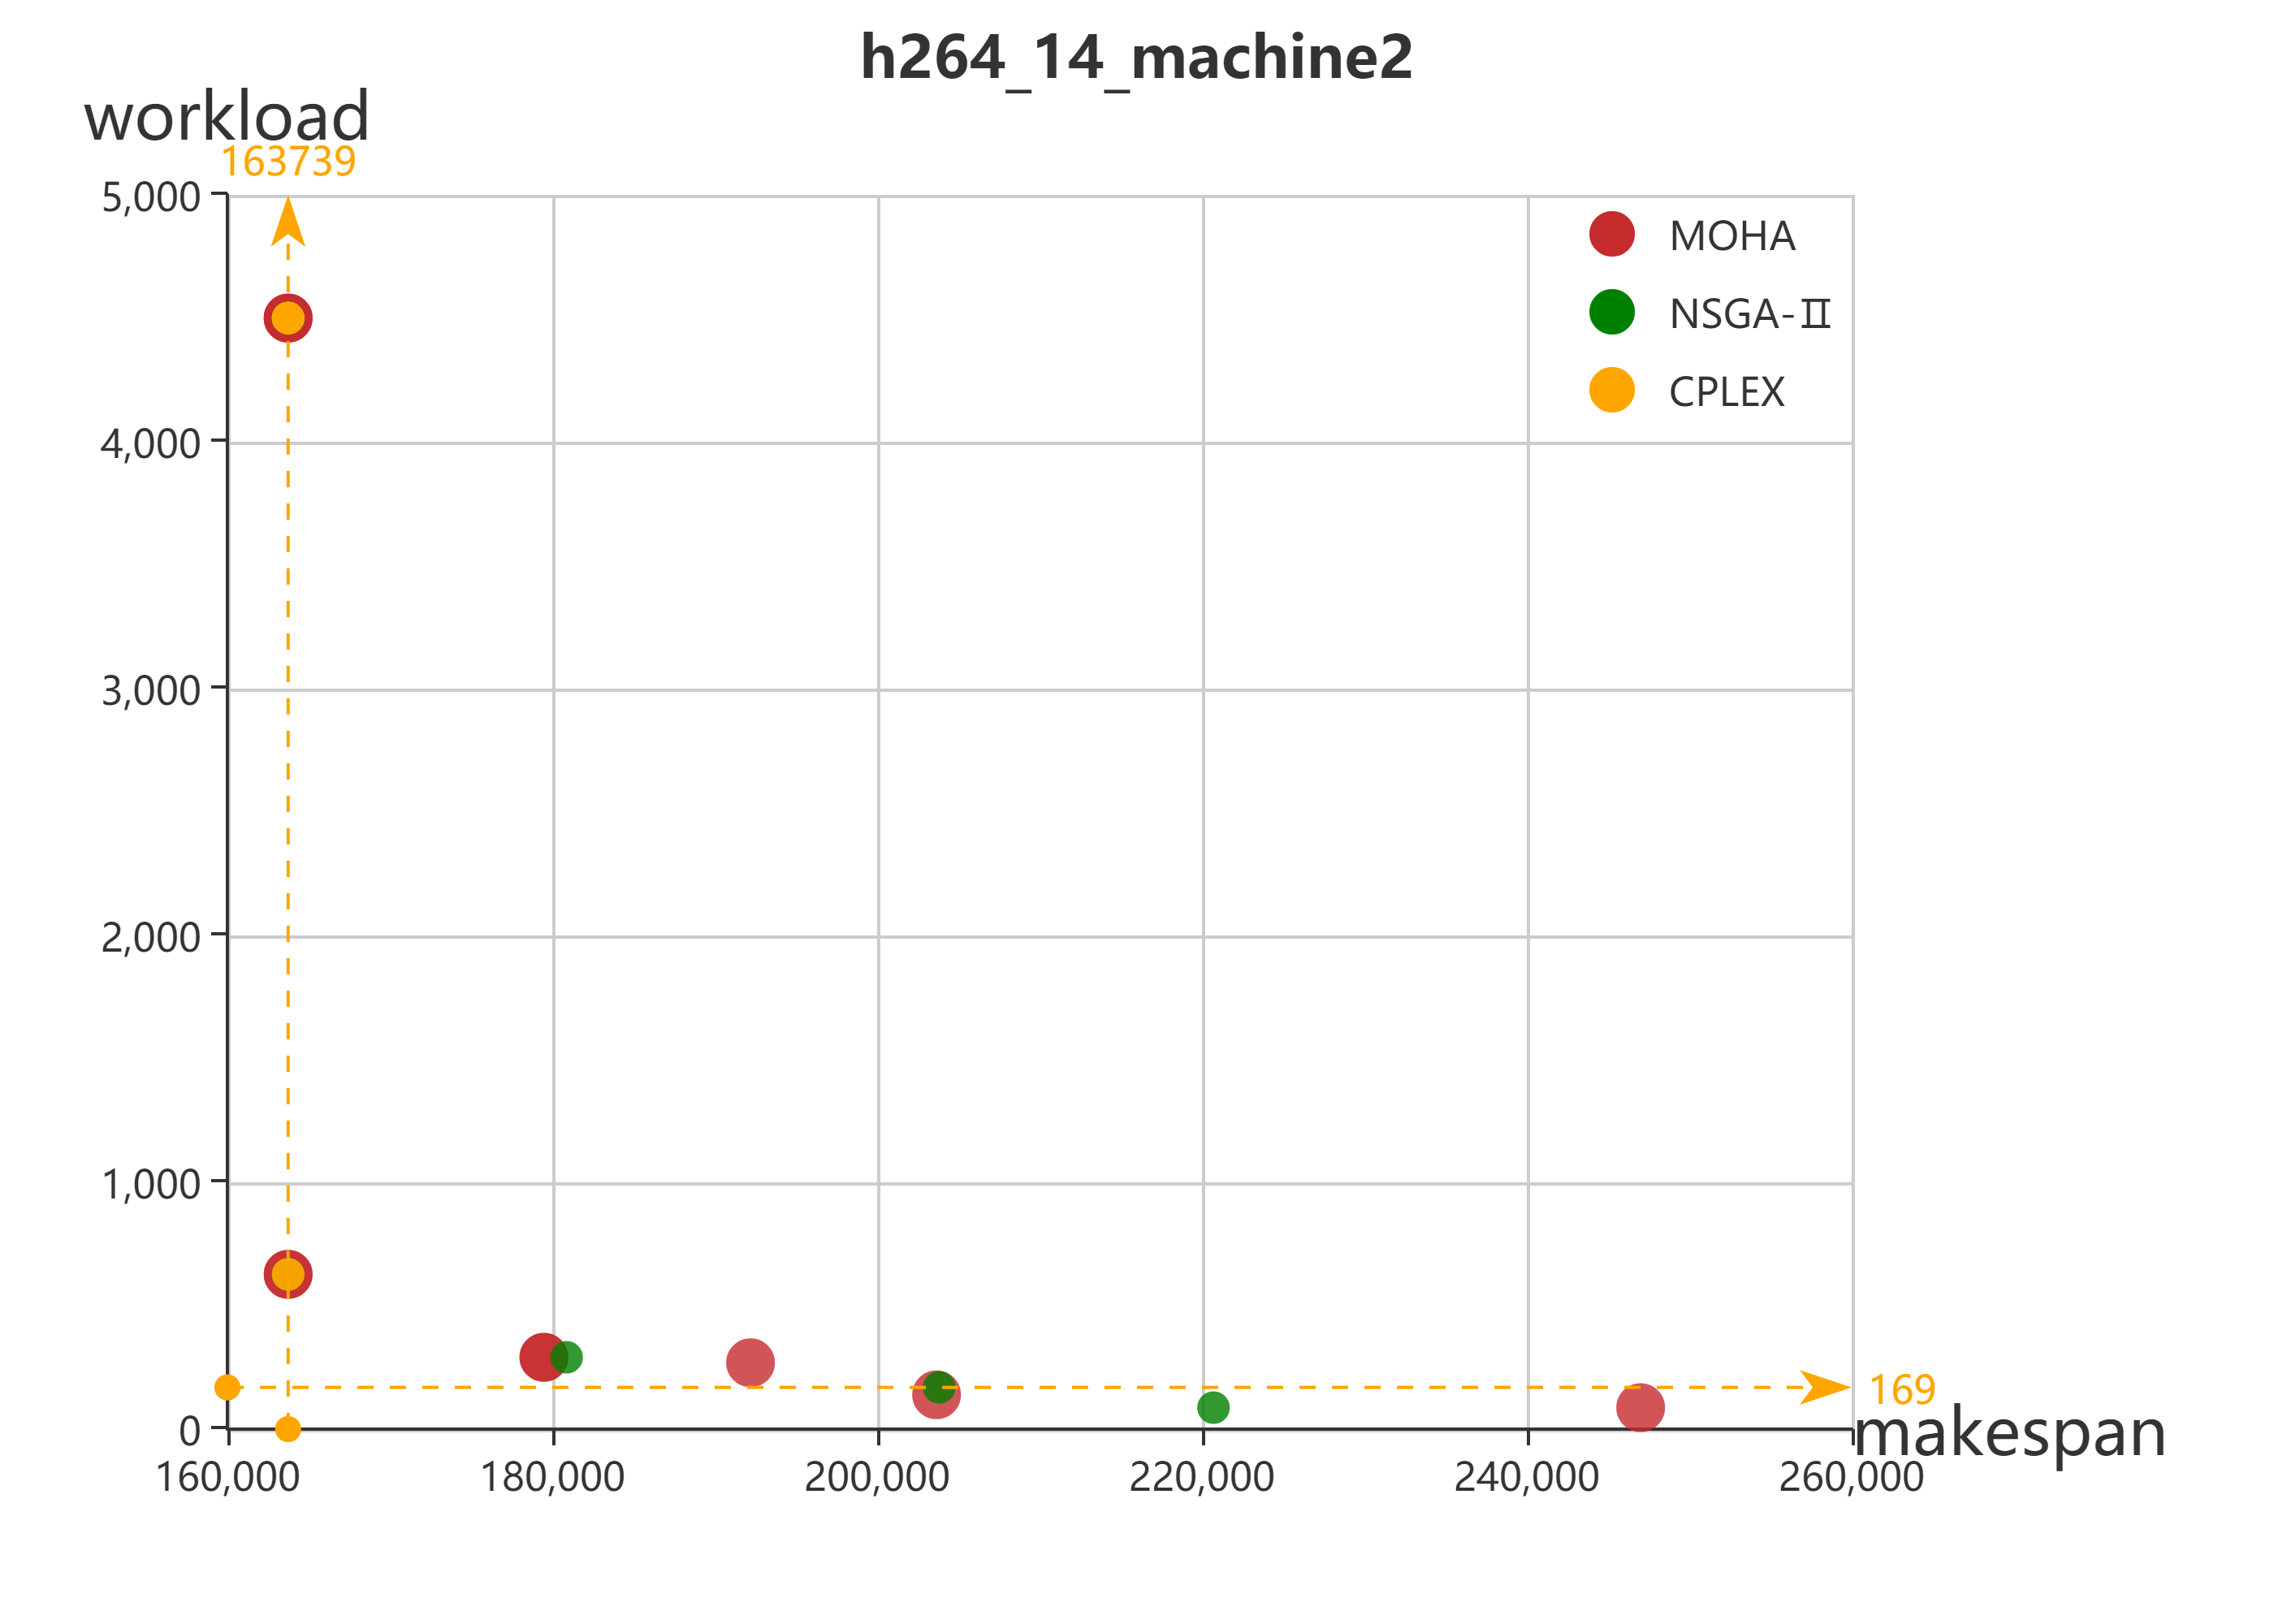
\includegraphics{./figures/h264_14_machine2}}}
\end{minipage}}%
\subfigure[H264 with 4 processors\label{fig:h264:2}]{
\begin{minipage}[b]{0.25\textwidth}
  \scalebox{0.045}{\rotatebox{0}{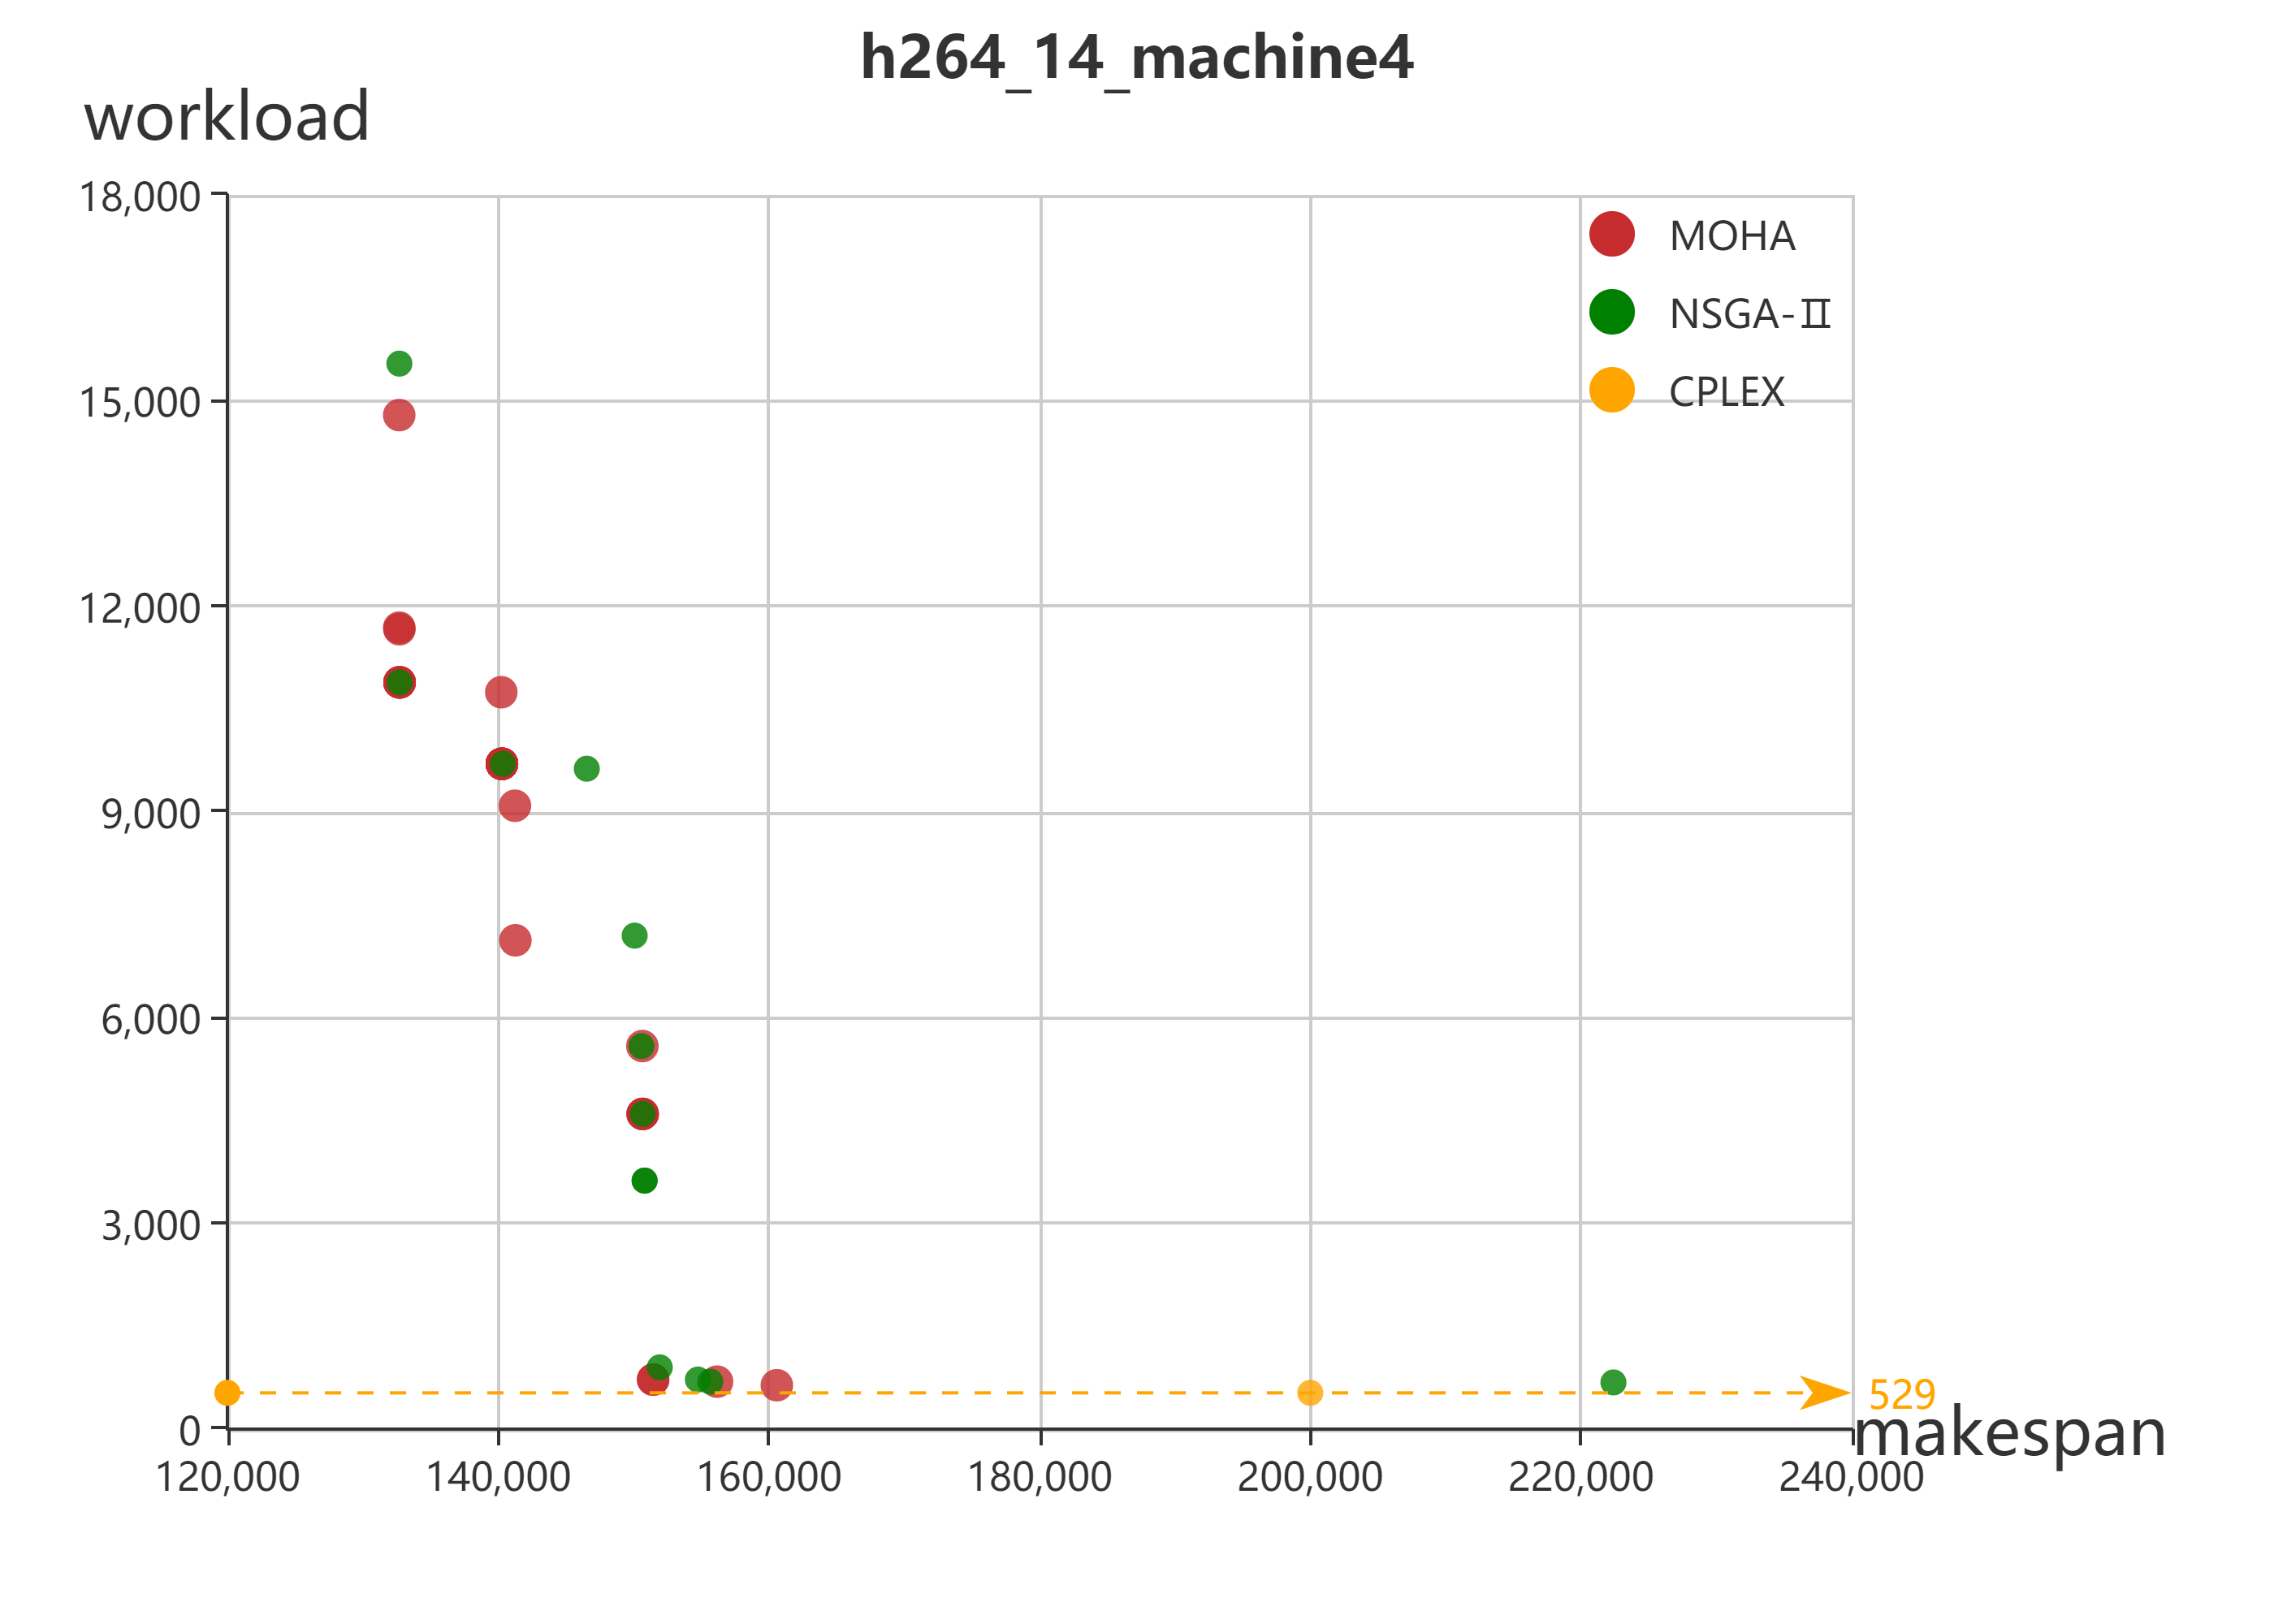
\includegraphics{./figures/h264_14_machine4}}}
\end{minipage}}
\caption{\label{fig:distribution} Distribution of final sets obtained by MOHA and NSGAII}
 \end{figure} 

%\begin{figure}[htp]
%\centering
%
%\subfigure[H264 with 2 processors\label{fig:h264}]{
% %\begin{minipage}[b]{0.25\textwidth}
%  \scalebox{0.065}{\rotatebox{0}{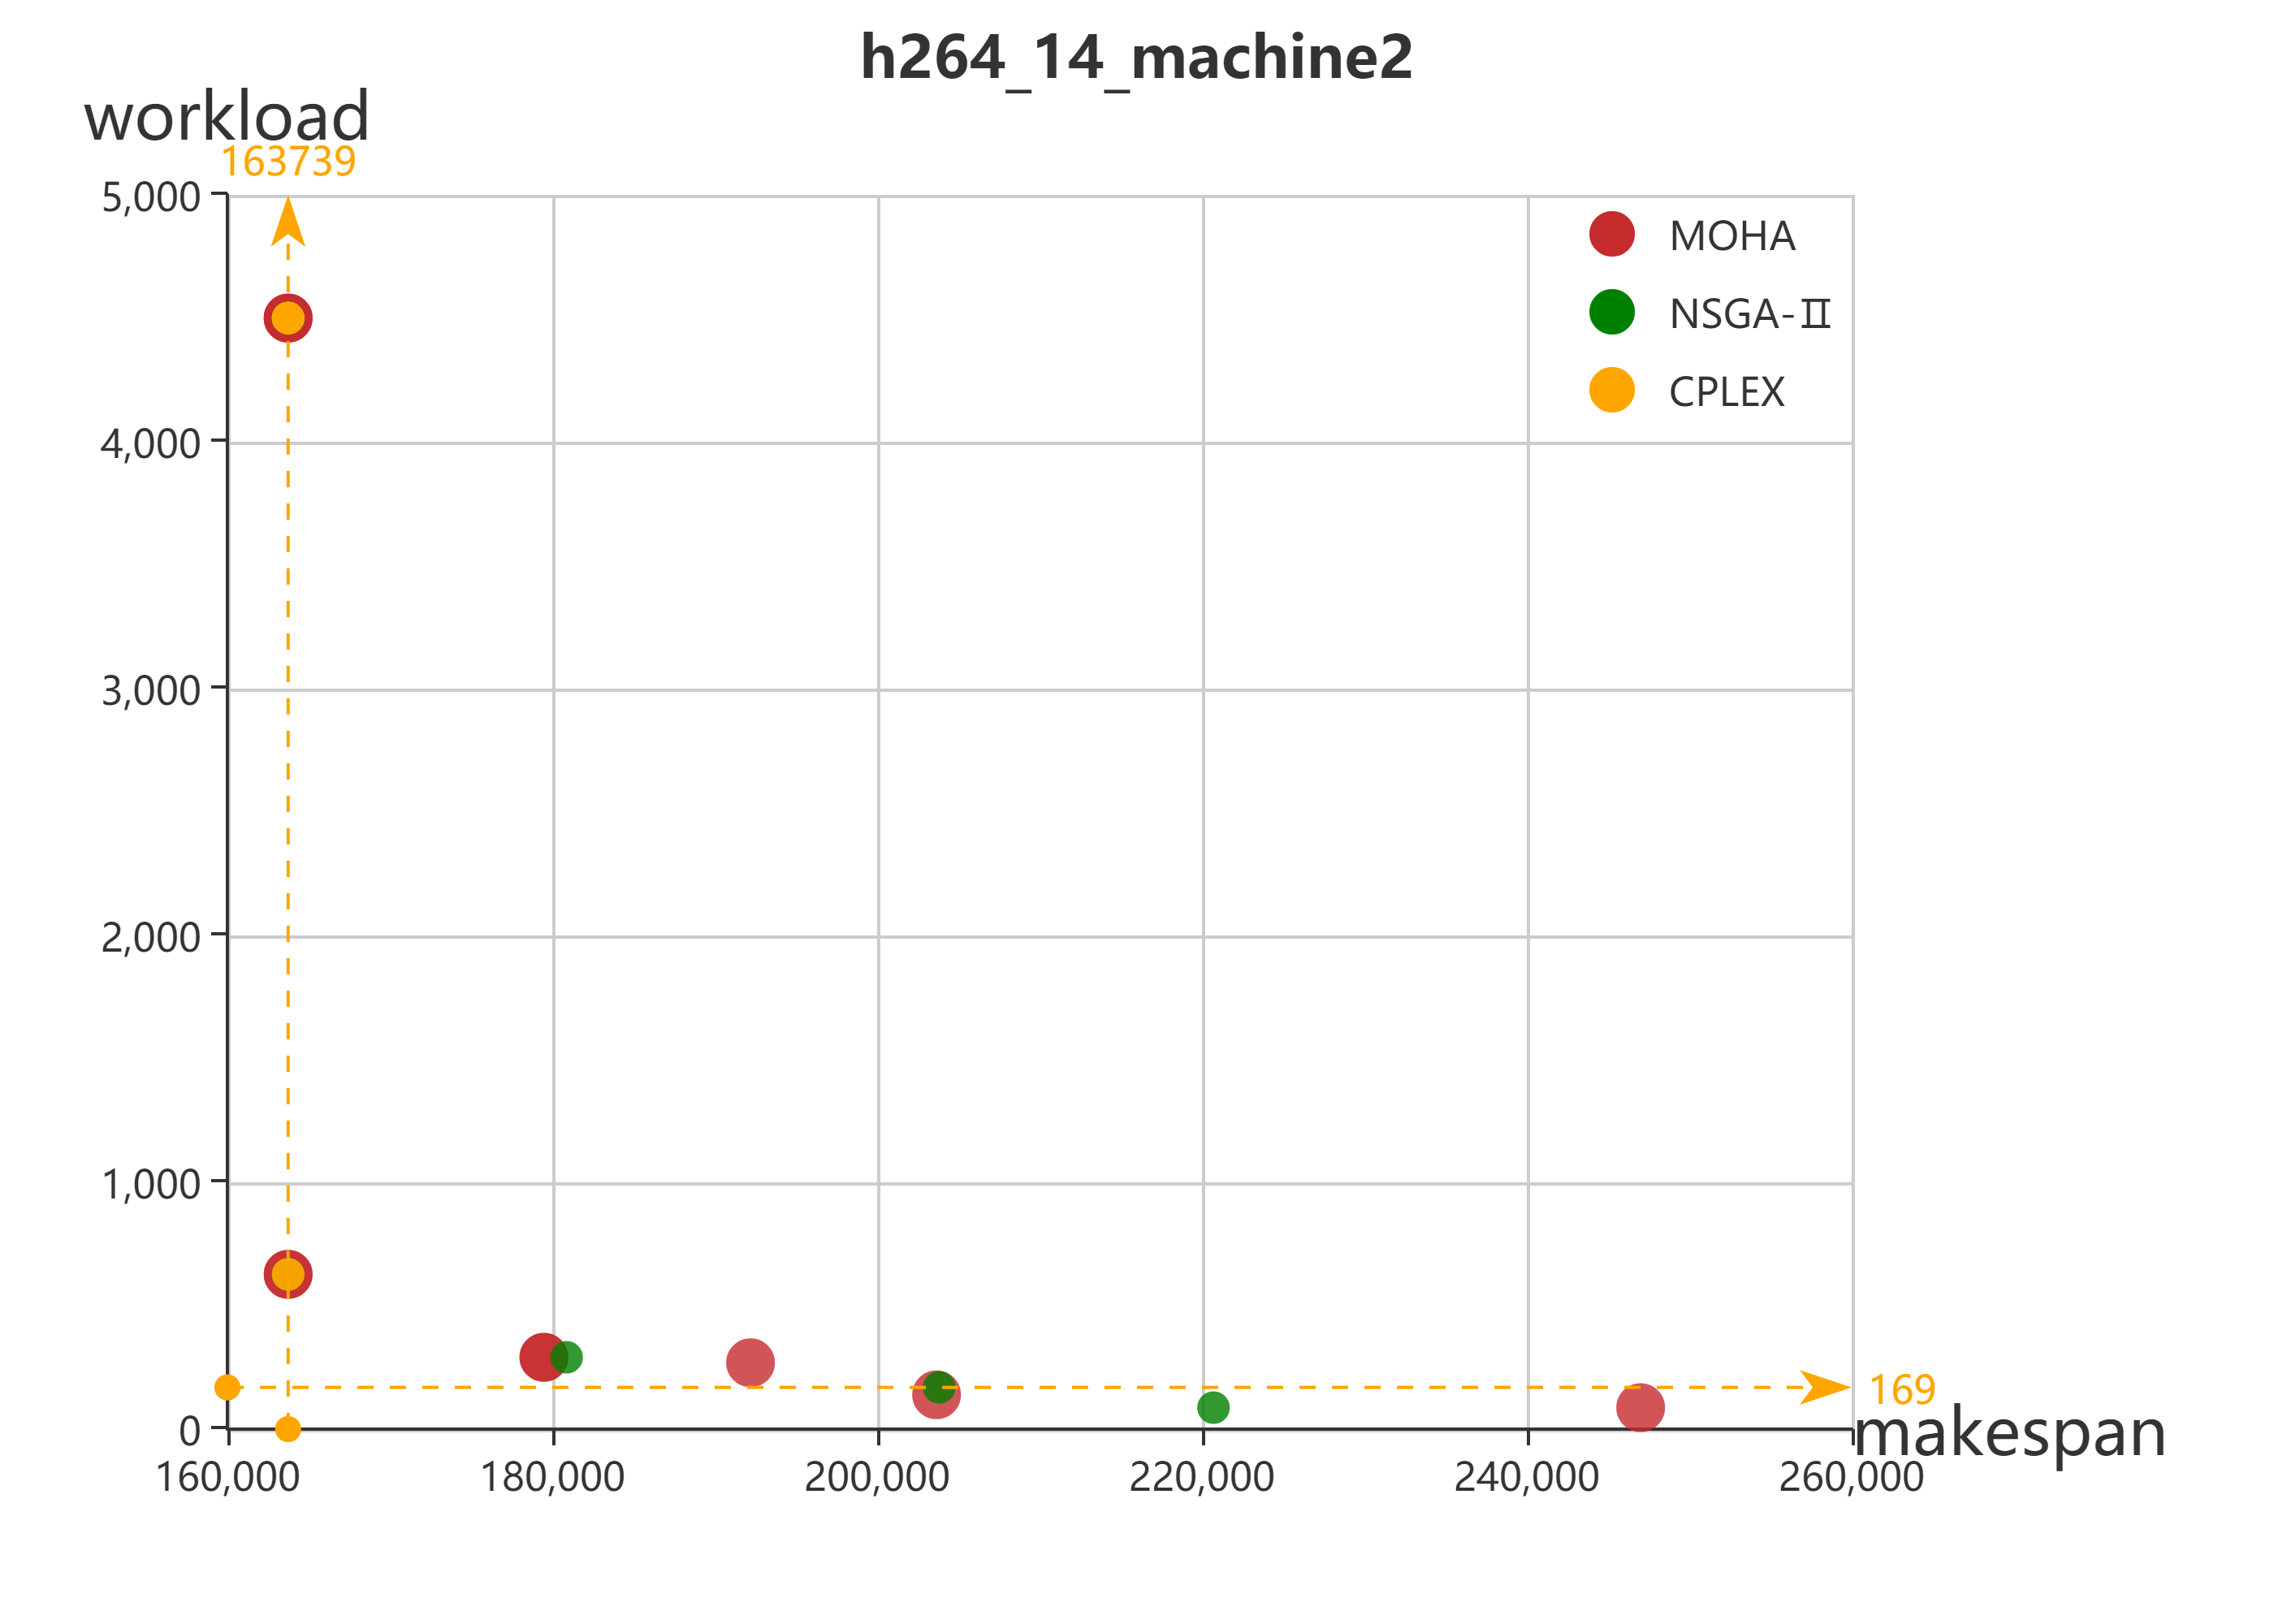
\includegraphics{./figures/h264_14_machine2}}}
%  }
%%\end{minipage}\
%\subfigure[H264 with 4 processors]{
%%\begin{minipage}[b]{0.25\textwidth}
%  \scalebox{0.065}{\rotatebox{0}{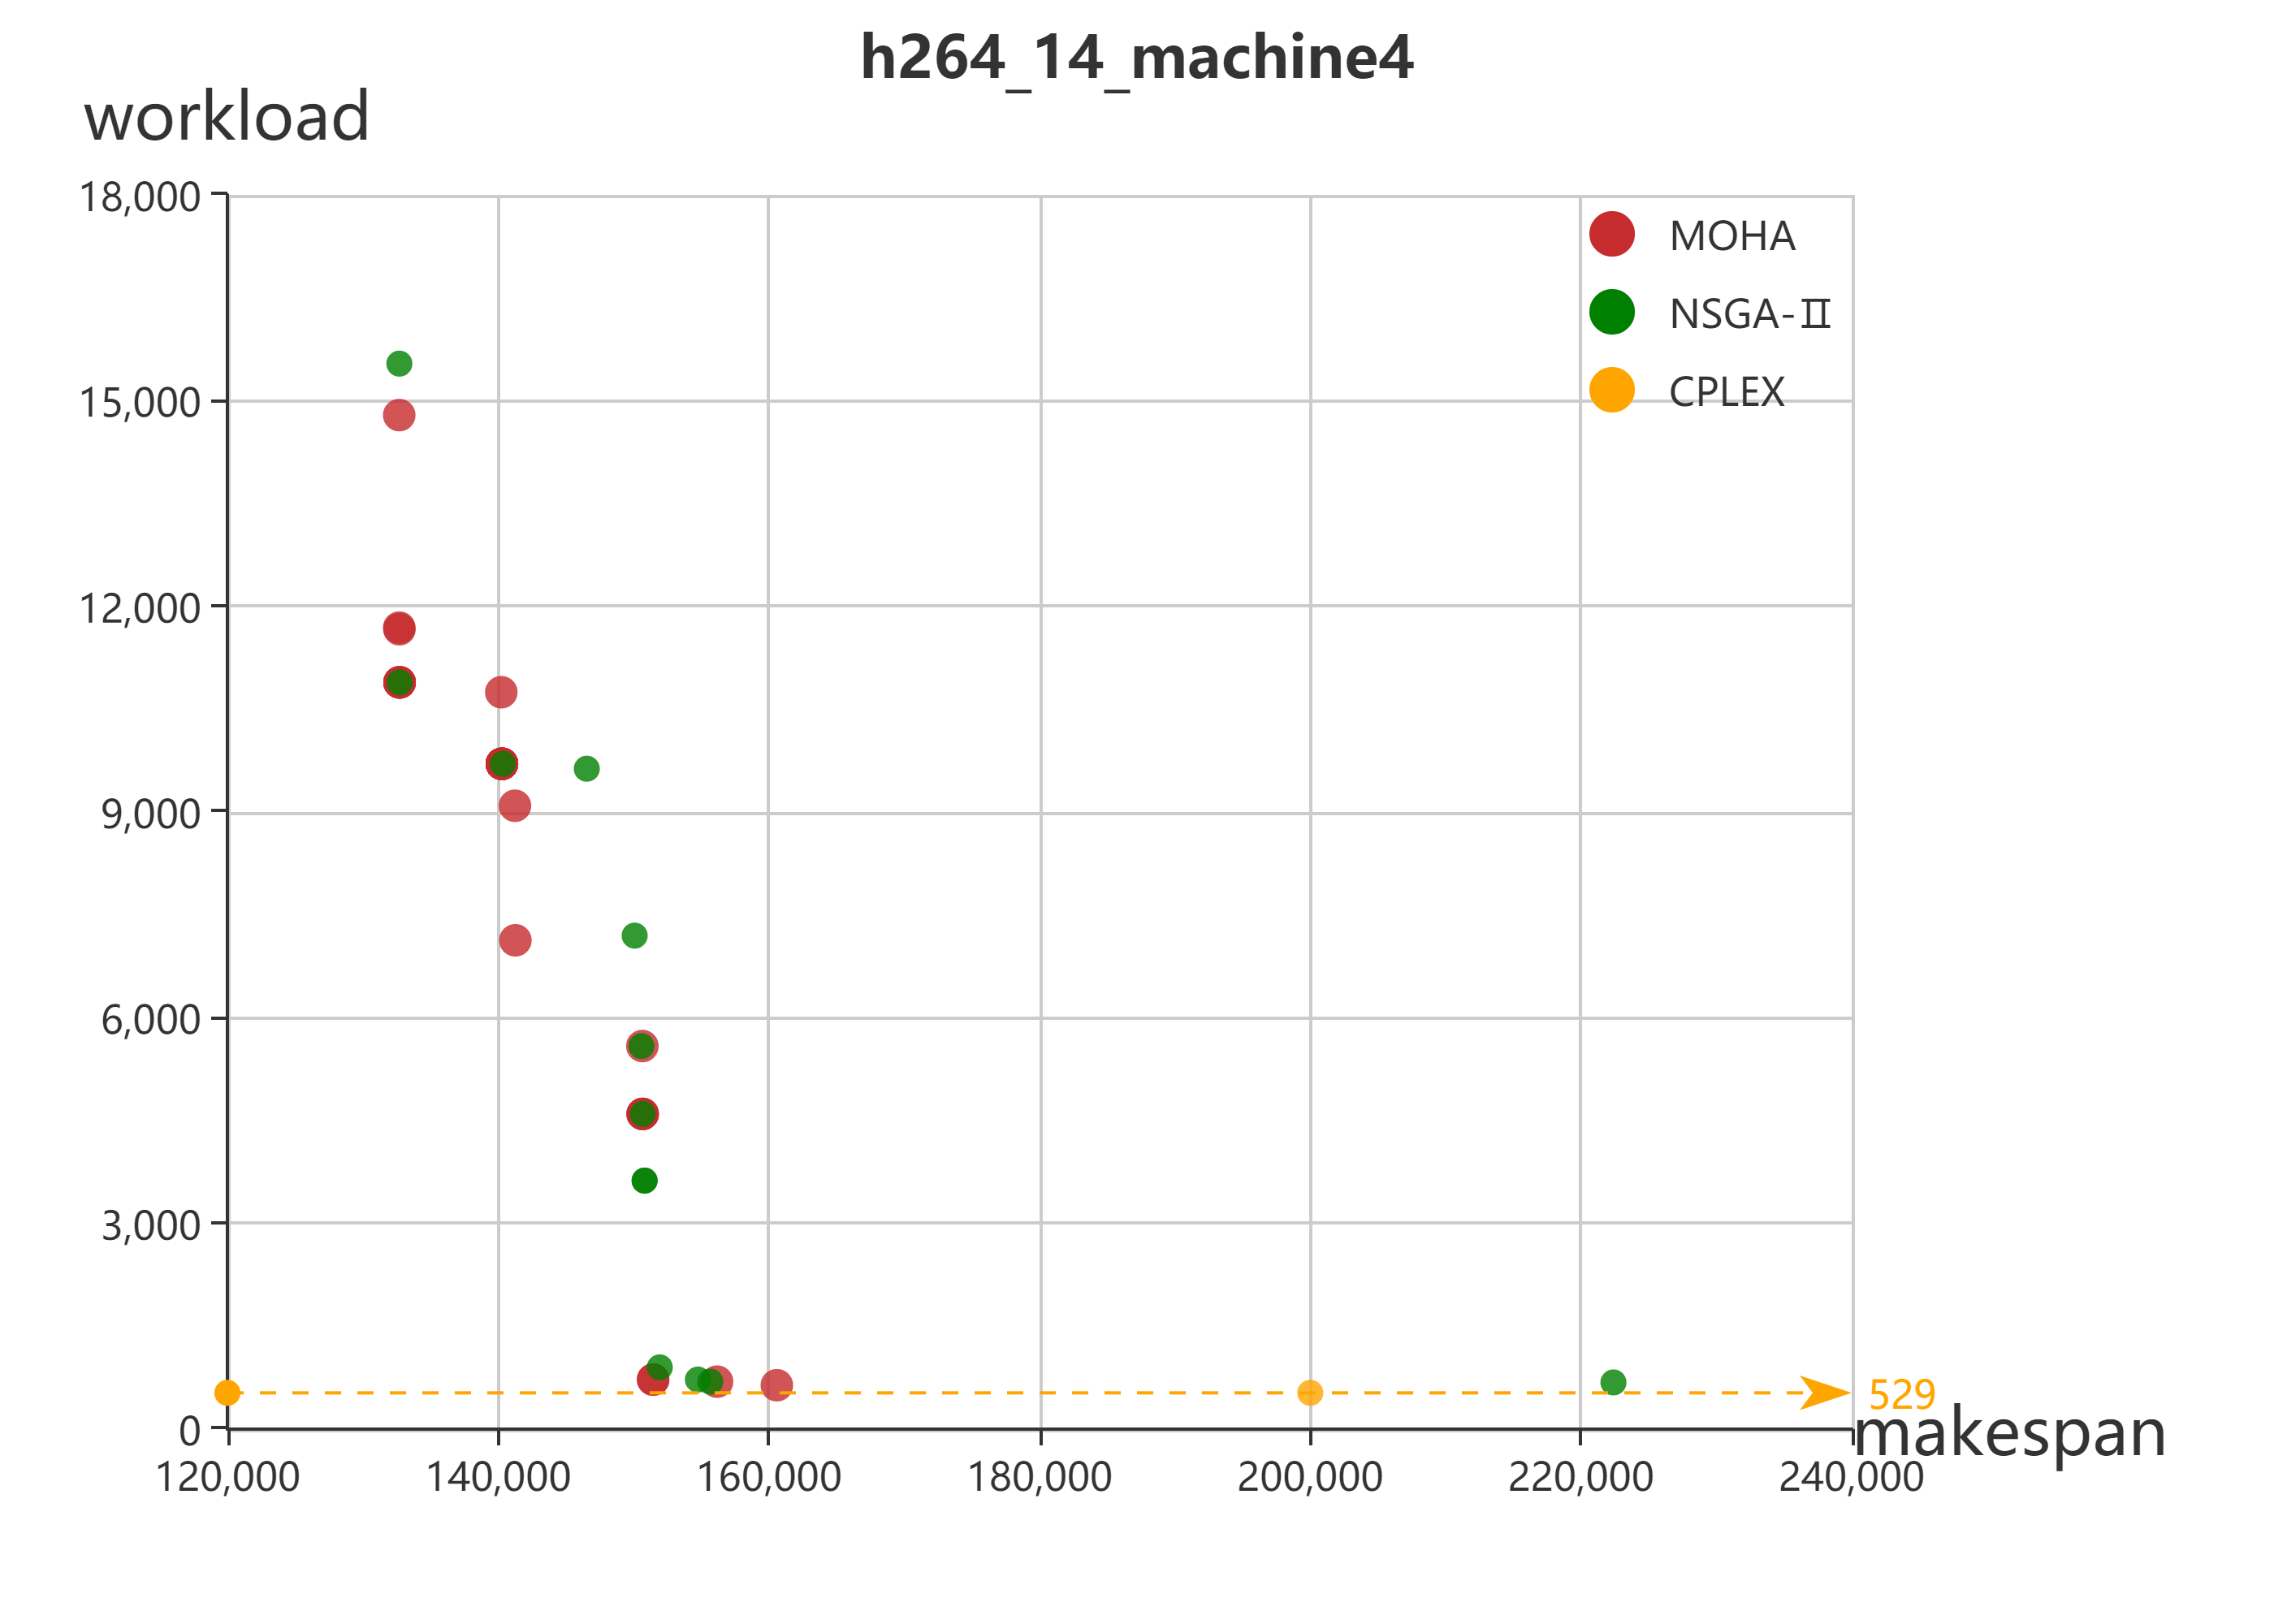
\includegraphics{./figures/h264_14_machine4}}}
%  
%%\end{minipage}}\
%}
%\caption{\label{fig:distribution}\rjnote Distribution of final sets obtained by MOHA and NSGAII}
% \end{figure} 

To evaluate the efficiency of our method, we have compared with the results from multi-objective evolutionary algorithm NSGAII~\cite{deb2002fast} and CPLEX over small scale examples. To compare with CPLEX, the two objectives are transformed into one by the introduced weights, whose ratios are sampled from (1:1) to (1:9999) and (9999:1) respectively. As the timeout of CPLEX is set to 2 hours, we could only obtain its results within the scale of 20 tasks and 2 processors.

%Two performance metrics are adopted to measure the effectiveness of the algorithm.
 
%The first one is an intuitive distribution of the non-dominated solutions which have been generated. 
The Pareto fronts\footnote{As the precedent relations are simple in these benchmarks, we could only obtain a few solutions in the Pareto fronts. } of the coarse-grained H264 decoder generated by MOHA, CPLEX and NSGAII, are illustrated in Fig. \ref{fig:distribution}. 
In the figure, the boundary of the two objectives are obtained by separated optimization for makespan and workload with CPLEX. 
And its Pareto fronts are calculated with various combination of weights.
%As Cplex can get only one solution after numerous of iterations, different weight combinations of the two objectives compose the Pareto front.
 %Also, the boundary of the two objectives are given by separately optimize makespan and workload using Cplex. 
We can observe that the results of MOHA are closer to the Pareto-front than that of NSGAII, and they can reach some boundaries computed by CPLEX. % on every benchmark. 

%What calls for special attention is that the dependency of tasks is so sequential in these instances that the pareto fronts only contain a few of solutions. However, it does not obstruct the observation of dominance.

Additional to the comparison from the figure, we also present the comparison from Set Coverage (C-metric), which reflects the degree of dominance is measured between different algorithms.
 Let \textit{X} and \textit{Y} be two approximations of the Pareto-front of a multi-objective problems. We define $C({A},{B})$ as the percentage of the solutions in \textit{B} that are dominated by at least one solution in \textit{A}, where
\begin{equation}
   C({A},{B})={\dfrac{u\in{B}|\exists v \in A: v \preceq u}{B}}.
\end{equation}
The higher $C({A},{B})$ is, the deeper extent $A$ dominates $B$.

The results of C-metric are listed in Table \ref{tab:cmetric}. $NA$ means the results are un-available within 2 hours.  As we can see, most solutions in MOHA dominate both NSGAII and CPLEX. 


%A second indicator called Set Coverage (C-metric) which reflects the degree of dominance is measured between MOHA and  NSGAII. Let \textit{X} and \textit{Y} be two approximations of the preto-front of an multi-objective problems,
%\begin{equation}
%   C({A},{B})={\dfrac{u\in{B}|\exists v \in A: v \preceq u}{B}}
%\end{equation}
%which is defined as the percentage of the solutions in \textit{B} that are dominated by at least one solution in \textit{A}. 
%/As Cplex can get only one solution after numerous of iterations, the metrics mentioned above are unapt. So, the third metric, \textit{W}(Cplex, MOHA), is whether the solution got by Cplex is dominated by the results of MOHA. In addition, the runtime \textit{Rtime} , solution numbers \emph{NumS} are also listed in TABLE \ref{tab:cplex}. The objective functions of Cplex are makespan and workload separately. That means for each instance, Cplex is run twice to optimize firstly the makespan and secondly the  workload. Results show that our proposed method gains no worse results than Cplex but spends less time in verse.
 
 \begin{table}[htp]\centering
\caption{Coverage Values between MOHA, CPLEX, NSGAII  \label{tab:cmetric}}%on six instances
\begin{lrbox}{\tablebox}
%\begin{scriptsize}
\begin{tabular}{|c|c|c|c|c|c|c|}
\hline

	\multirow{2}{*} {Benchmark} & \multirow{2}{*} {Tasks} & \multirow{2}{*} {Processors} & C(MOHA, & C(NSGAII,  & C(MOHA, & C(CPLEX,\\
	                  &           &               & NSGAII)  &  MOHA) & CPLEX) & MOHA) \\
\hline
	 \multirow{2}{*} {mp3decoder} &\multirow{2}{*}{16} & 2 & 0.8 & 0.2 & 1 & 0 \\
	 & & 4 & 0 & 0 & 1 & 0 \\ \hline
	\multirow{2}{*}{h264-14} & \multirow{2}{*}{14} & 2 & 0.4 & 0.17 & 0 & 0 \\
	& &   4 & 0.58 & 0.15 & 0 & 0\\ \hline
	\multirow{2}{*} {MWD} & \multirow{2}{*}{  12 } & 2 & 0 & 0 & 1 & 0\\
	& & 4 & 0 & 1 & 1 & 0\\\hline
	\multirow{2}{*}{TMNR} &\multirow{2}{*}{ 14 } & 2 & 0.67 & 0 & 0.5 & 0.5\\
	 && 4 & 0 & 0 & 0 &0.75\\\hline
	\multirow{2}{*}{FFT-loop} &\multirow{2}{*}{ 28} & 2 & 0.67 & 0.33 & 1 & 0\\

	& & 4 & 0 & 0.33 &NA &NA\\ \hline
	\multirow{2}{*}{FFT-butterfly} &\multirow{2}{*}{ 32} & 2  & 1 & 0 &NA &NA\\ 
        & 	& 4 & 1 &0 &NA &NA\\
%	mp3decoder & $ 16$ & 
%	h264-14 & $14$ & 4 & 0.58 & 0.15 & 0 & 0\\
%	MWD & $  12 $ & 4 & 0 & 1 & 1 & 0\\
%	TMNR & $ 14 $ & 4 & 0 & 0 & 0 &0.75\\
%	FFT-loop & $ 28 $ & 4 & 0 & 0.33 &NA &NA\\
%	FFT-butterfly & $ 32$ & 4 & 1 &0 &NA &NA\\
\hline
\end{tabular}	
%\end{scriptsize}
\end{lrbox}
\scalebox{0.65}{\usebox{\tablebox}}
\end{table}



% \begin{table}[htp]\centering
%\caption{Comparasion between Cplex and MOHA \label{tab:cplex}}
%\begin{lrbox}{\tablebox}
%\begin{tabular}{|c|c|c|c|c|}
%\hline
%	Dataset Name & Scale & W(Cplex, MOHA) & Rtime(s) & NumS %\\
%\hline
%	mp3decoder & $3 \ast 16$ & 0.75 & 0 & 1 \\
%	h264-14 & $2 \ast 14$ & 0.25 & 0.25 &1  \\
%	MWD & $3 \ast 12 $ & 1 & 0 & 1 \\
%	TMNR & $3 \ast 14 $ & 1 & 0 & 1 \\
%	FFT-loop & $2 \ast 28 $ & 1 & 0 &1 \\
%	FFT-butterfly & $2 \ast 32$ & 1 & 0 &1\\
%\hline
%\end{tabular}	
%\end{lrbox}
%\scalebox{0.9}{\usebox{\tablebox}}
%\end{table}
\subsection{ The scaliability of the MOHA algorithm}
\begin{figure}[htp]
\centering
	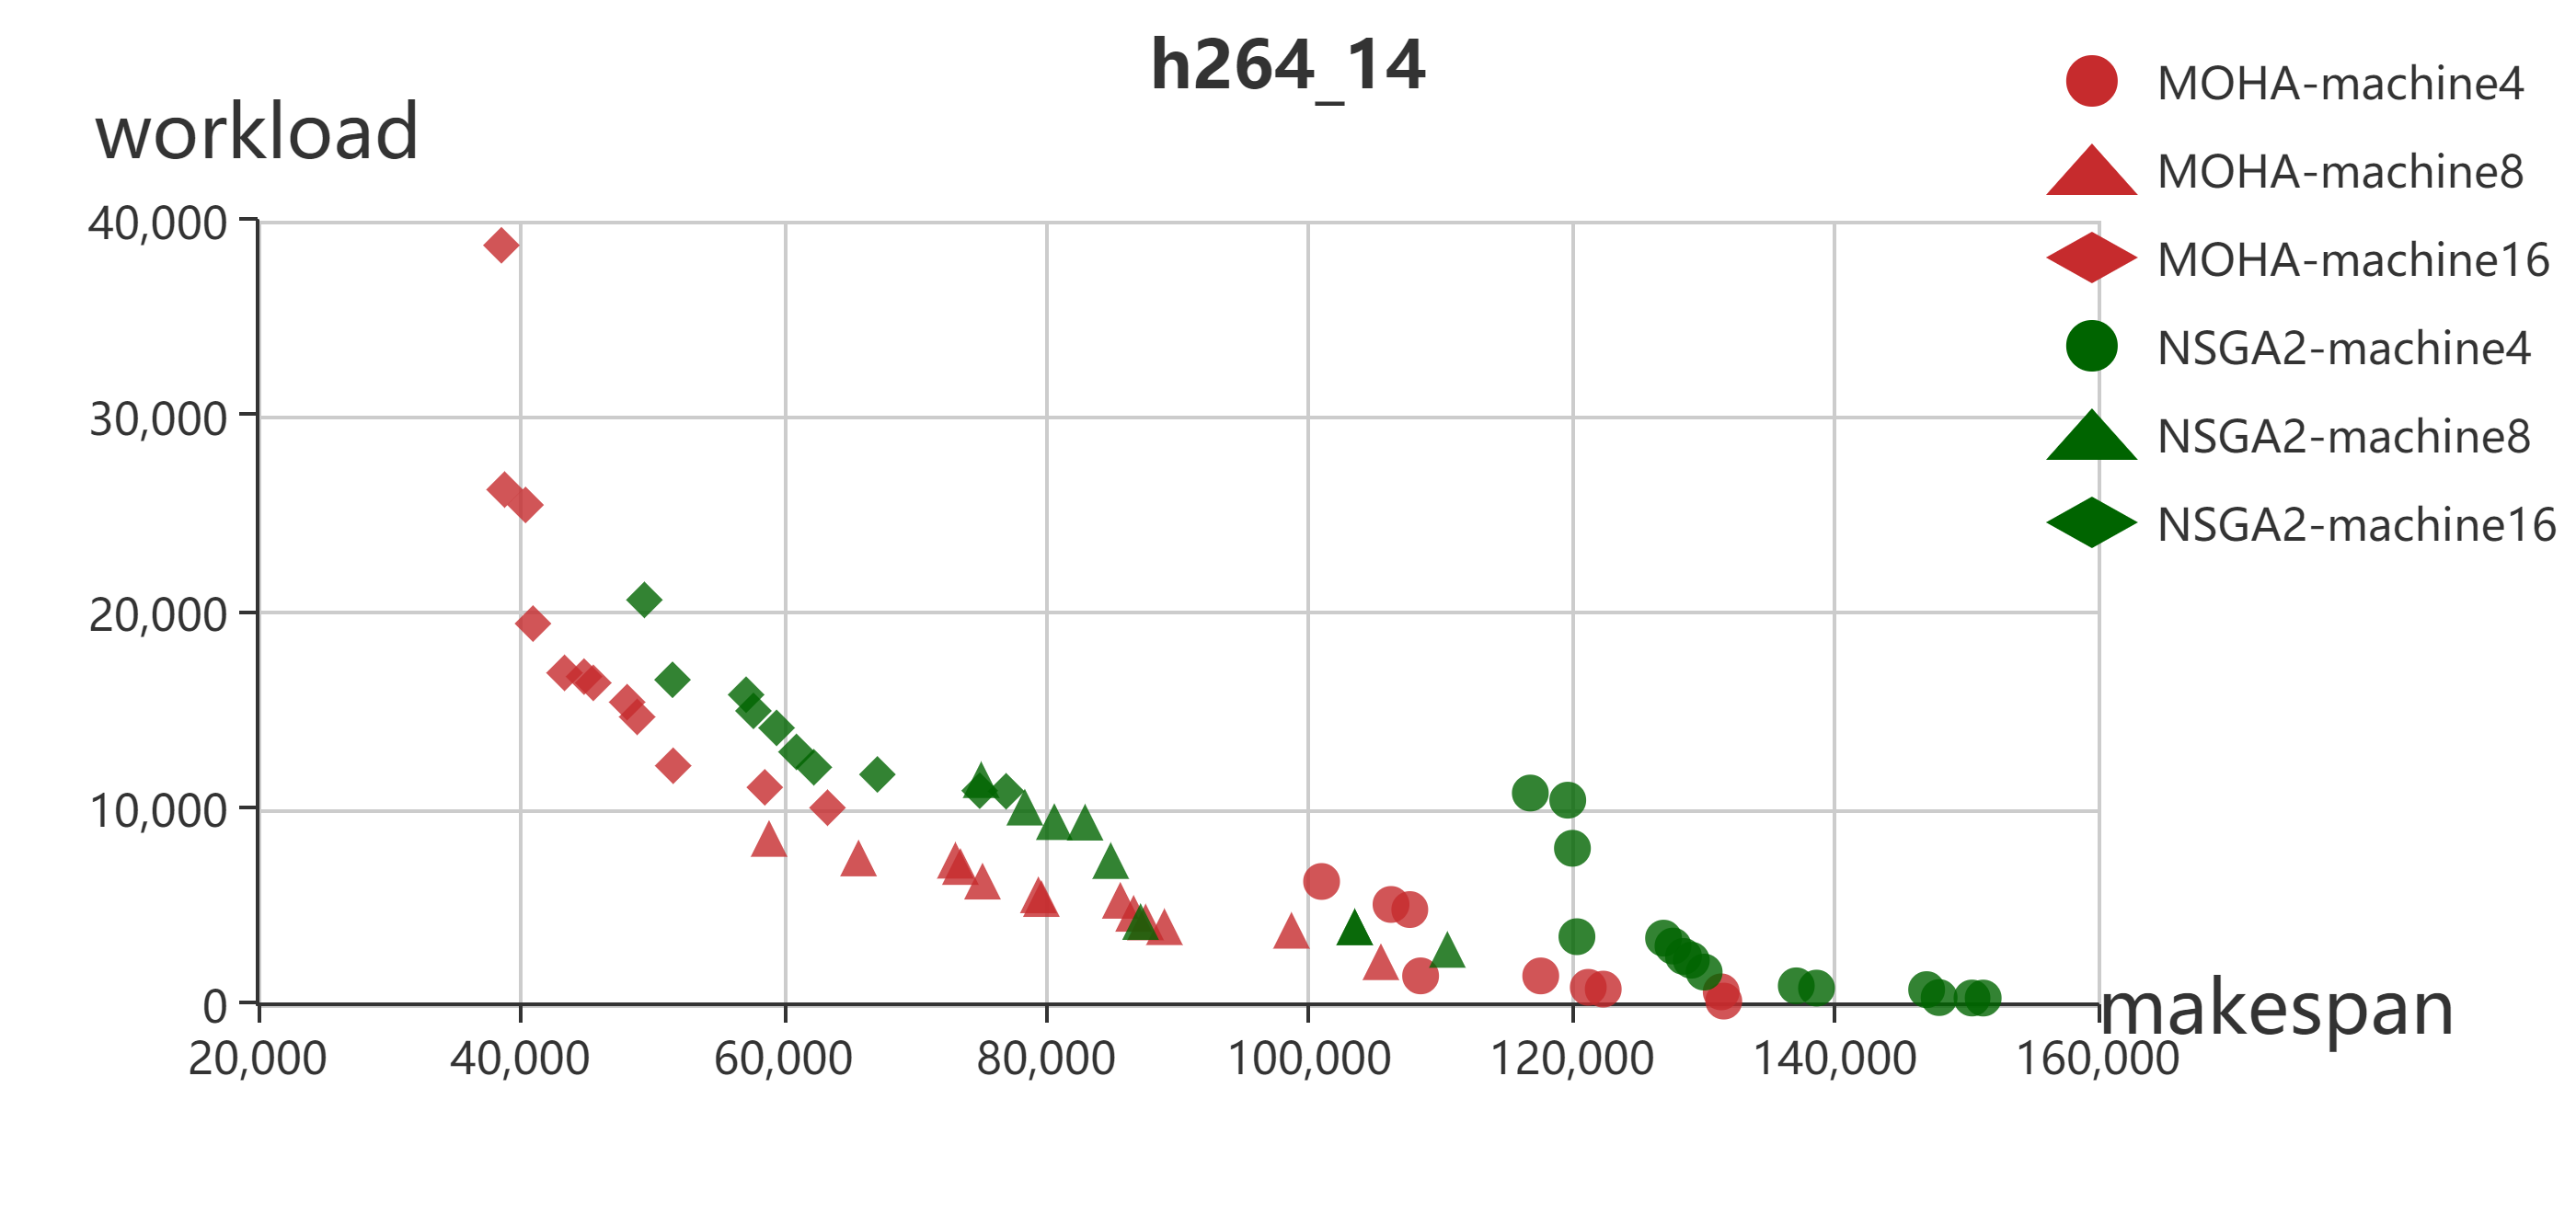
\includegraphics[width=0.9\columnwidth]{./figures/h264_14}
\caption{Distribution of final sets  for fine-grained H264}
 \label{fig:finegrained}
\vspace{-4mm}
 \end{figure} 
To show the scalability of our method, we have also evaluated the performance with the fine-grained H264 decoder example, with 264 tasks and 4, 8, 16 processors respectively. Its comparison with NSGAII is illustrated  in Fig. \ref{fig:finegrained}. The results show that MOHA can gain better results even on the large scale applications. 

%\subsection{Experimental Results}



\section{Conclusion and future work\label{se:con}}
To meet increasing requirements on  high  system performance and low power consumption, we have proposed two optimization objectives, i.e., makespan minimisation and workload balance, for mapping and scheduling problem of MPSoCs. The model for optimization encapsulates task scheduling, with the consideration of both computation and communication cost. To deal with the optimization of large scale applications, we have also proposed a multi-objective hybrid algorithm. Compared from the generated solutions, our algorithm outperforms  methods such as CPLEX and NSGAII.  
For the future work, we will refine the model to encompass more objectives to be optimized, as well as extending the current algorithm from two to more objectives optimization.  
\bibliographystyle{abbrv}
\bibliography{ilp}
\end{document}